\documentclass[twoside]{book}

% Packages required by doxygen
\usepackage{calc}
\usepackage{doxygen}
\usepackage{graphicx}
\usepackage[utf8]{inputenc}
\usepackage{makeidx}
\usepackage{multicol}
\usepackage{multirow}
\usepackage{textcomp}
\usepackage[table]{xcolor}

% Font selection
\usepackage[T1]{fontenc}
\usepackage{mathptmx}
\usepackage[scaled=.90]{helvet}
\usepackage{courier}
\usepackage{amssymb}
\usepackage{sectsty}
\renewcommand{\familydefault}{\sfdefault}
\allsectionsfont{%
  \fontseries{bc}\selectfont%
  \color{darkgray}%
}
\renewcommand{\DoxyLabelFont}{%
  \fontseries{bc}\selectfont%
  \color{darkgray}%
}

% Page & text layout
\usepackage{geometry}
\geometry{%
  a4paper,%
  top=2.5cm,%
  bottom=2.5cm,%
  left=2.5cm,%
  right=2.5cm%
}
\tolerance=750
\hfuzz=15pt
\hbadness=750
\setlength{\emergencystretch}{15pt}
\setlength{\parindent}{0cm}
\setlength{\parskip}{0.2cm}
\makeatletter
\renewcommand{\paragraph}{%
  \@startsection{paragraph}{4}{0ex}{-1.0ex}{1.0ex}{%
    \normalfont\normalsize\bfseries\SS@parafont%
  }%
}
\renewcommand{\subparagraph}{%
  \@startsection{subparagraph}{5}{0ex}{-1.0ex}{1.0ex}{%
    \normalfont\normalsize\bfseries\SS@subparafont%
  }%
}
\makeatother

% Headers & footers
\usepackage{fancyhdr}
\pagestyle{fancyplain}
\fancyhead[LE]{\fancyplain{}{\bfseries\thepage}}
\fancyhead[CE]{\fancyplain{}{}}
\fancyhead[RE]{\fancyplain{}{\bfseries\leftmark}}
\fancyhead[LO]{\fancyplain{}{\bfseries\rightmark}}
\fancyhead[CO]{\fancyplain{}{}}
\fancyhead[RO]{\fancyplain{}{\bfseries\thepage}}
\fancyfoot[LE]{\fancyplain{}{}}
\fancyfoot[CE]{\fancyplain{}{}}
\fancyfoot[RE]{\fancyplain{}{\bfseries\scriptsize Generated on Fri Jun 7 2013 16:18:10 for Camera Manager by Doxygen }}
\fancyfoot[LO]{\fancyplain{}{\bfseries\scriptsize Generated on Fri Jun 7 2013 16:18:10 for Camera Manager by Doxygen }}
\fancyfoot[CO]{\fancyplain{}{}}
\fancyfoot[RO]{\fancyplain{}{}}
\renewcommand{\footrulewidth}{0.4pt}
\renewcommand{\chaptermark}[1]{%
  \markboth{#1}{}%
}
\renewcommand{\sectionmark}[1]{%
  \markright{\thesection\ #1}%
}

% Indices & bibliography
\usepackage{natbib}
\usepackage[titles]{tocloft}
\setcounter{tocdepth}{3}
\setcounter{secnumdepth}{5}
\makeindex

% Hyperlinks (required, but should be loaded last)
\usepackage{ifpdf}
\ifpdf
  \usepackage[pdftex,pagebackref=true]{hyperref}
\else
  \usepackage[ps2pdf,pagebackref=true]{hyperref}
\fi
\hypersetup{%
  colorlinks=true,%
  linkcolor=blue,%
  citecolor=blue,%
  unicode%
}

% Custom commands
\newcommand{\clearemptydoublepage}{%
  \newpage{\pagestyle{empty}\cleardoublepage}%
}


%===== C O N T E N T S =====

\begin{document}

% Titlepage & ToC
\hypersetup{pageanchor=false}
\pagenumbering{roman}
\begin{titlepage}
\vspace*{7cm}
\begin{center}%
{\Large Camera Manager \\[1ex]\large 1.\-0 }\\
\vspace*{1cm}
{\large Generated by Doxygen 1.8.4}\\
\vspace*{0.5cm}
{\small Fri Jun 7 2013 16:18:10}\\
\end{center}
\end{titlepage}
\clearemptydoublepage
\tableofcontents
\clearemptydoublepage
\pagenumbering{arabic}
\hypersetup{pageanchor=true}

%--- Begin generated contents ---
\chapter{Hierarchical Index}
\section{Class Hierarchy}
This inheritance list is sorted roughly, but not completely, alphabetically\-:\begin{DoxyCompactList}
\item \contentsline{section}{Abstract\-Camera}{\pageref{class_abstract_camera}}{}
\begin{DoxyCompactList}
\item \contentsline{section}{Fly\-Camera}{\pageref{class_fly_camera}}{}
\item \contentsline{section}{Is\-Camera}{\pageref{class_is_camera}}{}
\item \contentsline{section}{Test\-Camera}{\pageref{class_test_camera}}{}
\end{DoxyCompactList}
\item \contentsline{section}{Camera\-Manager\-:\-:Camera\-Property}{\pageref{class_camera_manager_1_1_camera_property}}{}
\item Q\-Main\-Window\begin{DoxyCompactList}
\item \contentsline{section}{Main\-Window}{\pageref{class_main_window}}{}
\end{DoxyCompactList}
\item Q\-Object\begin{DoxyCompactList}
\item \contentsline{section}{Abstract\-Camera\-Manager}{\pageref{class_abstract_camera_manager}}{}
\begin{DoxyCompactList}
\item \contentsline{section}{Empty\-Camera\-Manager}{\pageref{class_empty_camera_manager}}{}
\item \contentsline{section}{Fly\-Camera\-Manager}{\pageref{class_fly_camera_manager}}{}
\item \contentsline{section}{Is\-Camera\-Manager}{\pageref{class_is_camera_manager}}{}
\item \contentsline{section}{Test\-Camera\-Manager}{\pageref{class_test_camera_manager}}{}
\end{DoxyCompactList}
\end{DoxyCompactList}
\item Q\-Widget\begin{DoxyCompactList}
\item \contentsline{section}{Q\-Video\-Widget}{\pageref{class_q_video_widget}}{}
\end{DoxyCompactList}
\end{DoxyCompactList}

\chapter{Class Index}
\section{Class List}
Here are the classes, structs, unions and interfaces with brief descriptions\-:\begin{DoxyCompactList}
\item\contentsline{section}{\hyperlink{class_abstract_camera}{Abstract\-Camera} \\*Class that need to be subclassed for each camera A\-P\-I. It is used to exchange Camera\-Property between the application and the A\-P\-I, to lauch auto capture and receive frames }{\pageref{class_abstract_camera}}{}
\item\contentsline{section}{\hyperlink{class_abstract_camera_manager}{Abstract\-Camera\-Manager} }{\pageref{class_abstract_camera_manager}}{}
\item\contentsline{section}{\hyperlink{class_camera_manager_1_1_camera_property}{Camera\-Manager\-::\-Camera\-Property} }{\pageref{class_camera_manager_1_1_camera_property}}{}
\item\contentsline{section}{\hyperlink{class_empty_camera_manager}{Empty\-Camera\-Manager} }{\pageref{class_empty_camera_manager}}{}
\item\contentsline{section}{\hyperlink{class_fly_camera}{Fly\-Camera} \\*The \hyperlink{class_fly_camera}{Fly\-Camera} class, represent a Fly\-Capture Camera with all its settings }{\pageref{class_fly_camera}}{}
\item\contentsline{section}{\hyperlink{class_fly_camera_manager}{Fly\-Camera\-Manager} \\*Deals with all the Fly Capture Cameras }{\pageref{class_fly_camera_manager}}{}
\item\contentsline{section}{\hyperlink{class_is_camera}{Is\-Camera} \\*The \hyperlink{class_is_camera}{Is\-Camera} class, represent a Image Source Camera with all its settings }{\pageref{class_is_camera}}{}
\item\contentsline{section}{\hyperlink{class_is_camera_manager}{Is\-Camera\-Manager} \\*The \hyperlink{class_fly_camera_manager}{Fly\-Camera\-Manager} class deals with all the Fly Capture Cameras }{\pageref{class_is_camera_manager}}{}
\item\contentsline{section}{\hyperlink{class_main_window}{Main\-Window} }{\pageref{class_main_window}}{}
\item\contentsline{section}{\hyperlink{class_q_video_widget}{Q\-Video\-Widget} }{\pageref{class_q_video_widget}}{}
\item\contentsline{section}{\hyperlink{class_test_camera}{Test\-Camera} }{\pageref{class_test_camera}}{}
\item\contentsline{section}{\hyperlink{class_test_camera_manager}{Test\-Camera\-Manager} }{\pageref{class_test_camera_manager}}{}
\end{DoxyCompactList}

\chapter{Class Documentation}
\hypertarget{class_abstract_camera}{\section{Abstract\-Camera Class Reference}
\label{class_abstract_camera}\index{Abstract\-Camera@{Abstract\-Camera}}
}


{\ttfamily \#include $<$abstractcamera.\-h$>$}

Inheritance diagram for Abstract\-Camera\-:\begin{figure}[H]
\begin{center}
\leavevmode
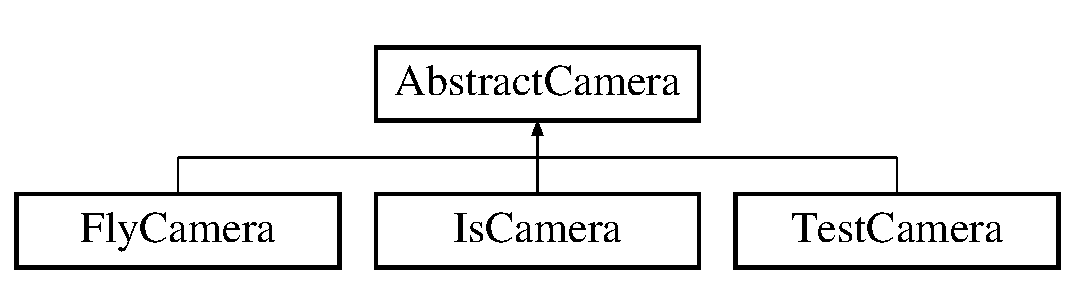
\includegraphics[height=2.000000cm]{class_abstract_camera}
\end{center}
\end{figure}
\subsection*{Public Member Functions}
\begin{DoxyCompactItemize}
\item 
virtual void \hyperlink{class_abstract_camera_a8b50d3e4925cfe74ed383376ba02bb5e}{set\-Property} (\hyperlink{class_camera_manager_1_1_camera_property}{Camera\-Manager\-::\-Camera\-Property} $\ast$p)=0
\begin{DoxyCompactList}\small\item\em set\-Property set the camera according to that property \end{DoxyCompactList}\item 
virtual void \hyperlink{class_abstract_camera_acb48ab701cd02e78604a3ca1c695b1cf}{update\-Property} (\hyperlink{class_camera_manager_1_1_camera_property}{Camera\-Manager\-::\-Camera\-Property} $\ast$p)=0
\begin{DoxyCompactList}\small\item\em update\-Property get the value of that property for that camera \end{DoxyCompactList}\item 
virtual bool \hyperlink{class_abstract_camera_a244917ab081c18caf389473847871dd6}{equals\-To} (\hyperlink{class_abstract_camera}{Abstract\-Camera} $\ast$c)
\begin{DoxyCompactList}\small\item\em equals\-To compare 2 cameras \end{DoxyCompactList}\item 
virtual std\-::string \hyperlink{class_abstract_camera_a75dc6b53d5a8717944d5e8ded9609611}{get\-String} ()=0
\begin{DoxyCompactList}\small\item\em get\-String get the name corresponding to the camera model and id \end{DoxyCompactList}\item 
\hypertarget{class_abstract_camera_a2f47d9877c5308856f42c94723faca33}{virtual void \hyperlink{class_abstract_camera_a2f47d9877c5308856f42c94723faca33}{start\-Auto\-Capture} ()=0}\label{class_abstract_camera_a2f47d9877c5308856f42c94723faca33}

\begin{DoxyCompactList}\small\item\em start\-Auto\-Capture start callback based Liveview \end{DoxyCompactList}\item 
\hypertarget{class_abstract_camera_a08bd5e2c3f8a92187f36e1f6322eccb5}{virtual void \hyperlink{class_abstract_camera_a08bd5e2c3f8a92187f36e1f6322eccb5}{stop\-Auto\-Capture} ()=0}\label{class_abstract_camera_a08bd5e2c3f8a92187f36e1f6322eccb5}

\begin{DoxyCompactList}\small\item\em stop\-Auto\-Capture stop callback based Liveview \end{DoxyCompactList}\item 
virtual Q\-Image \hyperlink{class_abstract_camera_aec58ab298b618632fd422cadd11bae17}{retrieve\-Image} ()=0
\begin{DoxyCompactList}\small\item\em retrieve\-Image get one image from camera \end{DoxyCompactList}\item 
void \hyperlink{class_abstract_camera_a19c1e4a98de744a5b8567b4764ceabe0}{start\-Capture} (\hyperlink{class_q_video_widget}{Q\-Video\-Widget} $\ast$video\-Widget)
\begin{DoxyCompactList}\small\item\em start\-Capture start liveview capture from manager \end{DoxyCompactList}\end{DoxyCompactItemize}
\subsection*{Protected Member Functions}
\begin{DoxyCompactItemize}
\item 
void \hyperlink{class_abstract_camera_a8fa5df9ffe74c0df6e1b8d74b6bf3b9d}{send\-Frame} (Q\-Image img)
\begin{DoxyCompactList}\small\item\em send\-Frame send a new Q\-Image for the view \end{DoxyCompactList}\end{DoxyCompactItemize}


\subsection{Detailed Description}
\hyperlink{class_abstract_camera}{Abstract\-Camera} Class that need to be subclassed for each camera A\-P\-I used to exchange Camera\-Property between the application and the A\-P\-I 

\subsection{Member Function Documentation}
\hypertarget{class_abstract_camera_a244917ab081c18caf389473847871dd6}{\index{Abstract\-Camera@{Abstract\-Camera}!equals\-To@{equals\-To}}
\index{equals\-To@{equals\-To}!AbstractCamera@{Abstract\-Camera}}
\subsubsection[{equals\-To}]{\setlength{\rightskip}{0pt plus 5cm}bool Abstract\-Camera\-::equals\-To (
\begin{DoxyParamCaption}
\item[{{\bf Abstract\-Camera} $\ast$}]{c}
\end{DoxyParamCaption}
)\hspace{0.3cm}{\ttfamily [virtual]}}}\label{class_abstract_camera_a244917ab081c18caf389473847871dd6}


equals\-To compare 2 cameras 


\begin{DoxyParams}{Parameters}
{\em c} & camera to compare \\
\hline
\end{DoxyParams}
\begin{DoxyReturn}{Returns}
true if the cameras are physically the same 
\end{DoxyReturn}


Reimplemented in \hyperlink{class_fly_camera_a8121735229105485f73289a36bd41042}{Fly\-Camera}, and \hyperlink{class_is_camera_acb734c645fa0c5e4ffc64001b87daa0d}{Is\-Camera}.

\hypertarget{class_abstract_camera_a75dc6b53d5a8717944d5e8ded9609611}{\index{Abstract\-Camera@{Abstract\-Camera}!get\-String@{get\-String}}
\index{get\-String@{get\-String}!AbstractCamera@{Abstract\-Camera}}
\subsubsection[{get\-String}]{\setlength{\rightskip}{0pt plus 5cm}virtual std\-::string Abstract\-Camera\-::get\-String (
\begin{DoxyParamCaption}
{}
\end{DoxyParamCaption}
)\hspace{0.3cm}{\ttfamily [pure virtual]}}}\label{class_abstract_camera_a75dc6b53d5a8717944d5e8ded9609611}


get\-String get the name corresponding to the camera model and id 

\begin{DoxyReturn}{Returns}
String containing these informations 
\end{DoxyReturn}


Implemented in \hyperlink{class_fly_camera_a97938fec7396d02574383f7db50d9e58}{Fly\-Camera}, \hyperlink{class_is_camera_af0791bc3cdb5d552fb6f73285b467408}{Is\-Camera}, and \hyperlink{class_test_camera_a5ddb007a4c0c44e06b24787298f1c97c}{Test\-Camera}.

\hypertarget{class_abstract_camera_aec58ab298b618632fd422cadd11bae17}{\index{Abstract\-Camera@{Abstract\-Camera}!retrieve\-Image@{retrieve\-Image}}
\index{retrieve\-Image@{retrieve\-Image}!AbstractCamera@{Abstract\-Camera}}
\subsubsection[{retrieve\-Image}]{\setlength{\rightskip}{0pt plus 5cm}virtual Q\-Image Abstract\-Camera\-::retrieve\-Image (
\begin{DoxyParamCaption}
{}
\end{DoxyParamCaption}
)\hspace{0.3cm}{\ttfamily [pure virtual]}}}\label{class_abstract_camera_aec58ab298b618632fd422cadd11bae17}


retrieve\-Image get one image from camera 

\begin{DoxyReturn}{Returns}
Q\-Image image 
\end{DoxyReturn}


Implemented in \hyperlink{class_fly_camera_a0e935d2f7d21e31e470670ff5b6740e1}{Fly\-Camera}, \hyperlink{class_is_camera_abd737cee4788d70a4614d8ea6ea883d2}{Is\-Camera}, and \hyperlink{class_test_camera_a283bd75f1b9500e35ba7aa252c2df14e}{Test\-Camera}.

\hypertarget{class_abstract_camera_a8fa5df9ffe74c0df6e1b8d74b6bf3b9d}{\index{Abstract\-Camera@{Abstract\-Camera}!send\-Frame@{send\-Frame}}
\index{send\-Frame@{send\-Frame}!AbstractCamera@{Abstract\-Camera}}
\subsubsection[{send\-Frame}]{\setlength{\rightskip}{0pt plus 5cm}void Abstract\-Camera\-::send\-Frame (
\begin{DoxyParamCaption}
\item[{Q\-Image}]{img}
\end{DoxyParamCaption}
)\hspace{0.3cm}{\ttfamily [protected]}}}\label{class_abstract_camera_a8fa5df9ffe74c0df6e1b8d74b6bf3b9d}


send\-Frame send a new Q\-Image for the view 


\begin{DoxyParams}{Parameters}
{\em img} & Q\-Image grabbed from the camera \\
\hline
\end{DoxyParams}
\hypertarget{class_abstract_camera_a8b50d3e4925cfe74ed383376ba02bb5e}{\index{Abstract\-Camera@{Abstract\-Camera}!set\-Property@{set\-Property}}
\index{set\-Property@{set\-Property}!AbstractCamera@{Abstract\-Camera}}
\subsubsection[{set\-Property}]{\setlength{\rightskip}{0pt plus 5cm}virtual void Abstract\-Camera\-::set\-Property (
\begin{DoxyParamCaption}
\item[{{\bf Camera\-Manager\-::\-Camera\-Property} $\ast$}]{p}
\end{DoxyParamCaption}
)\hspace{0.3cm}{\ttfamily [pure virtual]}}}\label{class_abstract_camera_a8b50d3e4925cfe74ed383376ba02bb5e}


set\-Property set the camera according to that property 


\begin{DoxyParams}{Parameters}
{\em p} & property to set \\
\hline
\end{DoxyParams}


Implemented in \hyperlink{class_fly_camera_ad9d4102cab167f0d5739b2af808c43ee}{Fly\-Camera}, \hyperlink{class_is_camera_a70c90a32bde9fcc3c594a526c7cba33c}{Is\-Camera}, and \hyperlink{class_test_camera_a92507f0e4601f93912b06297e4b59d99}{Test\-Camera}.

\hypertarget{class_abstract_camera_a19c1e4a98de744a5b8567b4764ceabe0}{\index{Abstract\-Camera@{Abstract\-Camera}!start\-Capture@{start\-Capture}}
\index{start\-Capture@{start\-Capture}!AbstractCamera@{Abstract\-Camera}}
\subsubsection[{start\-Capture}]{\setlength{\rightskip}{0pt plus 5cm}void Abstract\-Camera\-::start\-Capture (
\begin{DoxyParamCaption}
\item[{{\bf Q\-Video\-Widget} $\ast$}]{video\-Widget}
\end{DoxyParamCaption}
)}}\label{class_abstract_camera_a19c1e4a98de744a5b8567b4764ceabe0}


start\-Capture start liveview capture from manager 


\begin{DoxyParams}{Parameters}
{\em label} & wil update the label with images from the camera \\
\hline
\end{DoxyParams}
\hypertarget{class_abstract_camera_acb48ab701cd02e78604a3ca1c695b1cf}{\index{Abstract\-Camera@{Abstract\-Camera}!update\-Property@{update\-Property}}
\index{update\-Property@{update\-Property}!AbstractCamera@{Abstract\-Camera}}
\subsubsection[{update\-Property}]{\setlength{\rightskip}{0pt plus 5cm}virtual void Abstract\-Camera\-::update\-Property (
\begin{DoxyParamCaption}
\item[{{\bf Camera\-Manager\-::\-Camera\-Property} $\ast$}]{p}
\end{DoxyParamCaption}
)\hspace{0.3cm}{\ttfamily [pure virtual]}}}\label{class_abstract_camera_acb48ab701cd02e78604a3ca1c695b1cf}


update\-Property get the value of that property for that camera 


\begin{DoxyParams}{Parameters}
{\em p} & property to update \\
\hline
\end{DoxyParams}


Implemented in \hyperlink{class_fly_camera_a8f87a0d8ccbee558e629189e2c8ab271}{Fly\-Camera}, \hyperlink{class_is_camera_a5e2c484168c627eb79d61658e880300d}{Is\-Camera}, and \hyperlink{class_test_camera_a6b0c9e25baafe0a8d211b32851cb67b3}{Test\-Camera}.



The documentation for this class was generated from the following files\-:\begin{DoxyCompactItemize}
\item 
C\-:/\-Users/\-V1rgul/\-Git\-Hub/\-Project-\/\-Norway/\-Projet\-Norvege/abstractcamera.\-h\item 
C\-:/\-Users/\-V1rgul/\-Git\-Hub/\-Project-\/\-Norway/\-Projet\-Norvege/abstractcamera.\-cpp\end{DoxyCompactItemize}

\hypertarget{class_abstract_camera_manager}{\section{Abstract\-Camera\-Manager Class Reference}
\label{class_abstract_camera_manager}\index{Abstract\-Camera\-Manager@{Abstract\-Camera\-Manager}}
}
Inheritance diagram for Abstract\-Camera\-Manager\-:\begin{figure}[H]
\begin{center}
\leavevmode
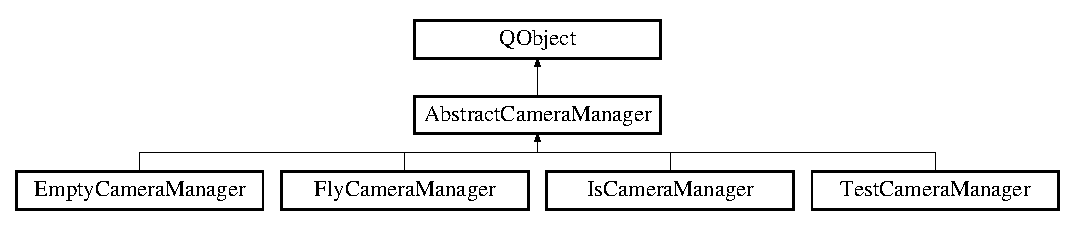
\includegraphics[height=2.592592cm]{class_abstract_camera_manager}
\end{center}
\end{figure}
\subsection*{Public Member Functions}
\begin{DoxyCompactItemize}
\item 
virtual void \hyperlink{class_abstract_camera_manager_a8e215b2531fd8c18551382dc8f571817}{detect\-New\-Cameras} (std\-::vector$<$ \hyperlink{class_abstract_camera}{Abstract\-Camera} $\ast$ $>$ $\ast$new\-Cameras)=0
\begin{DoxyCompactList}\small\item\em detect\-New\-Cameras (Pure virtual) detect new cameras \end{DoxyCompactList}\item 
virtual std\-::string \hyperlink{class_abstract_camera_manager_a6e4b041842471b9ed42ddd5c9ab260d1}{get\-Name} () const =0
\begin{DoxyCompactList}\small\item\em get\-Name (Pure virtual) get the name of the Manager \end{DoxyCompactList}\item 
Q\-Model\-Index \hyperlink{class_abstract_camera_manager_a609f8e3af887c5652ccf9a37d4e133c1}{detect\-New\-Cameras\-And\-Expand} ()
\begin{DoxyCompactList}\small\item\em detect\-New\-Cameras\-And\-Expand detect new cameras \end{DoxyCompactList}\item 
\hypertarget{class_abstract_camera_manager_a336e5cf760314194c1baf1234b87b247}{void {\bfseries update\-Images} ()}\label{class_abstract_camera_manager_a336e5cf760314194c1baf1234b87b247}

\item 
\hypertarget{class_abstract_camera_manager_a518b8dd27c032030ff23930488da0a52}{void {\bfseries update\-Properties} ()}\label{class_abstract_camera_manager_a518b8dd27c032030ff23930488da0a52}

\item 
Q\-Model\-Index \hyperlink{class_abstract_camera_manager_a4eaaf63434076e5d53d19a44f434bec9}{add\-Group} ()
\begin{DoxyCompactList}\small\item\em add\-Group add a empty group of cameras in the model \end{DoxyCompactList}\item 
void \hyperlink{class_abstract_camera_manager_a5eea7f4d2ab3ea314020b405550b378c}{remove\-Group} (Q\-Model\-Index index)
\begin{DoxyCompactList}\small\item\em remove\-Group remove a group from the model \end{DoxyCompactList}\item 
void \hyperlink{class_abstract_camera_manager_a89cd0d1f9bb47d4abda51ea4f1e08f49}{reset\-Item} (Q\-Model\-Index index)
\begin{DoxyCompactList}\small\item\em resetitem reset the name of a camera \end{DoxyCompactList}\item 
void \hyperlink{class_abstract_camera_manager_aeafa7b5e2b0eb5bbc105fe6a0ee5e2f2}{activate\-Camera} (\hyperlink{class_abstract_camera}{Abstract\-Camera} $\ast$camera, Q\-Standard\-Item $\ast$item, bool active)
\begin{DoxyCompactList}\small\item\em activate\-Camera check the camera in the model, add it in the active\-Cameras vector and open a subwindow for it \end{DoxyCompactList}\item 
\hypertarget{class_abstract_camera_manager_a92ed218ecaab3f6a75d3d24e5544d17f}{void \hyperlink{class_abstract_camera_manager_a92ed218ecaab3f6a75d3d24e5544d17f}{desactive\-All\-Cameras} ()}\label{class_abstract_camera_manager_a92ed218ecaab3f6a75d3d24e5544d17f}

\begin{DoxyCompactList}\small\item\em desactive\-All\-Cameras used to close all liveviews from this manager \end{DoxyCompactList}\item 
void \hyperlink{class_abstract_camera_manager_a10dee0f2e9a5efa1cf8b5775df66fb19}{camera\-Tree\-\_\-item\-Clicked} (const Q\-Model\-Index \&index, Q\-String \&string, int \&icon, bool \&editable, bool \&deleteable)
\begin{DoxyCompactList}\small\item\em camera\-Tree\-\_\-item\-Clicked select a camera or a group to edit its properties \end{DoxyCompactList}\item 
\hypertarget{class_abstract_camera_manager_a01cbc0e517b10e8b1c087138307ab676}{void {\bfseries activate\-Live\-View} (bool active)}\label{class_abstract_camera_manager_a01cbc0e517b10e8b1c087138307ab676}

\item 
Q\-Standard\-Item\-Model $\ast$ \hyperlink{class_abstract_camera_manager_a02097102061955f0092969a6cf812823}{get\-Model} ()
\begin{DoxyCompactList}\small\item\em get\-Model get the model ( camera list ) \end{DoxyCompactList}\item 
Q\-Tree\-Widget $\ast$ \hyperlink{class_abstract_camera_manager_a8cfcc9f2156936f1d8faea55ad97eeab}{get\-Properties\-Widget} ()
\begin{DoxyCompactList}\small\item\em get\-Properties\-Widget get the model of the properties \end{DoxyCompactList}\item 
void \hyperlink{class_abstract_camera_manager_a9369df77518a91e24596d2bbe3436bab}{set\-Main\-Window} (\hyperlink{class_main_window}{Main\-Window} $\ast$window)
\begin{DoxyCompactList}\small\item\em set\-Main\-Window to set the needed cross reference \end{DoxyCompactList}\end{DoxyCompactItemize}
\subsection*{Protected Member Functions}
\begin{DoxyCompactItemize}
\item 
\hyperlink{class_abstract_camera_manager_a23be9d93959d992c91efcf1416c597ef}{Abstract\-Camera\-Manager} (bool empty=false)
\begin{DoxyCompactList}\small\item\em \hyperlink{class_abstract_camera_manager}{Abstract\-Camera\-Manager} constructor. \end{DoxyCompactList}\item 
void \hyperlink{class_abstract_camera_manager_ac5c7ff3b69138df82efafa0400b50ce5}{set\-Properties} (std\-::vector$<$ \hyperlink{class_camera_manager_1_1_camera_property}{Camera\-Manager\-::\-Camera\-Property} $>$ \&properties)
\begin{DoxyCompactList}\small\item\em set\-Properties add properties tha can be set and retrieved to/from cameras for this A\-P\-I \end{DoxyCompactList}\end{DoxyCompactItemize}


\subsection{Constructor \& Destructor Documentation}
\hypertarget{class_abstract_camera_manager_a23be9d93959d992c91efcf1416c597ef}{\index{Abstract\-Camera\-Manager@{Abstract\-Camera\-Manager}!Abstract\-Camera\-Manager@{Abstract\-Camera\-Manager}}
\index{Abstract\-Camera\-Manager@{Abstract\-Camera\-Manager}!AbstractCameraManager@{Abstract\-Camera\-Manager}}
\subsubsection[{Abstract\-Camera\-Manager}]{\setlength{\rightskip}{0pt plus 5cm}Abstract\-Camera\-Manager\-::\-Abstract\-Camera\-Manager (
\begin{DoxyParamCaption}
\item[{bool}]{empty = {\ttfamily false}}
\end{DoxyParamCaption}
)\hspace{0.3cm}{\ttfamily [protected]}}}\label{class_abstract_camera_manager_a23be9d93959d992c91efcf1416c597ef}


\hyperlink{class_abstract_camera_manager}{Abstract\-Camera\-Manager} constructor. 


\begin{DoxyParams}{Parameters}
{\em empty} & true if the manager is an emty manager \\
\hline
\end{DoxyParams}


\subsection{Member Function Documentation}
\hypertarget{class_abstract_camera_manager_aeafa7b5e2b0eb5bbc105fe6a0ee5e2f2}{\index{Abstract\-Camera\-Manager@{Abstract\-Camera\-Manager}!activate\-Camera@{activate\-Camera}}
\index{activate\-Camera@{activate\-Camera}!AbstractCameraManager@{Abstract\-Camera\-Manager}}
\subsubsection[{activate\-Camera}]{\setlength{\rightskip}{0pt plus 5cm}void Abstract\-Camera\-Manager\-::activate\-Camera (
\begin{DoxyParamCaption}
\item[{{\bf Abstract\-Camera} $\ast$}]{camera, }
\item[{Q\-Standard\-Item $\ast$}]{item, }
\item[{bool}]{active}
\end{DoxyParamCaption}
)}}\label{class_abstract_camera_manager_aeafa7b5e2b0eb5bbc105fe6a0ee5e2f2}


activate\-Camera check the camera in the model, add it in the active\-Cameras vector and open a subwindow for it 


\begin{DoxyParams}{Parameters}
{\em camera} & pointer to the camera to add \\
\hline
{\em item} & position of the camera in the model \\
\hline
{\em active} & true to activate, false to desactivate \\
\hline
\end{DoxyParams}
\hypertarget{class_abstract_camera_manager_a4eaaf63434076e5d53d19a44f434bec9}{\index{Abstract\-Camera\-Manager@{Abstract\-Camera\-Manager}!add\-Group@{add\-Group}}
\index{add\-Group@{add\-Group}!AbstractCameraManager@{Abstract\-Camera\-Manager}}
\subsubsection[{add\-Group}]{\setlength{\rightskip}{0pt plus 5cm}Q\-Model\-Index Abstract\-Camera\-Manager\-::add\-Group (
\begin{DoxyParamCaption}
{}
\end{DoxyParamCaption}
)}}\label{class_abstract_camera_manager_a4eaaf63434076e5d53d19a44f434bec9}


add\-Group add a empty group of cameras in the model 

\begin{DoxyReturn}{Returns}
the index in the model corresponding to this group, in order to select it 
\end{DoxyReturn}
\hypertarget{class_abstract_camera_manager_a10dee0f2e9a5efa1cf8b5775df66fb19}{\index{Abstract\-Camera\-Manager@{Abstract\-Camera\-Manager}!camera\-Tree\-\_\-item\-Clicked@{camera\-Tree\-\_\-item\-Clicked}}
\index{camera\-Tree\-\_\-item\-Clicked@{camera\-Tree\-\_\-item\-Clicked}!AbstractCameraManager@{Abstract\-Camera\-Manager}}
\subsubsection[{camera\-Tree\-\_\-item\-Clicked}]{\setlength{\rightskip}{0pt plus 5cm}void Abstract\-Camera\-Manager\-::camera\-Tree\-\_\-item\-Clicked (
\begin{DoxyParamCaption}
\item[{const Q\-Model\-Index \&}]{index, }
\item[{Q\-String \&}]{string, }
\item[{int \&}]{icon, }
\item[{bool \&}]{editable, }
\item[{bool \&}]{deleteable}
\end{DoxyParamCaption}
)}}\label{class_abstract_camera_manager_a10dee0f2e9a5efa1cf8b5775df66fb19}


camera\-Tree\-\_\-item\-Clicked select a camera or a group to edit its properties 


\begin{DoxyParams}{Parameters}
{\em index} & index of the item in the model \\
\hline
{\em string} & desccritive of the item \\
\hline
{\em icon} & corresponding to the type of element selected \\
\hline
{\em editable} & true if the item is editable \\
\hline
{\em deletable} & true if the item is deletable \\
\hline
\end{DoxyParams}
\hypertarget{class_abstract_camera_manager_a8e215b2531fd8c18551382dc8f571817}{\index{Abstract\-Camera\-Manager@{Abstract\-Camera\-Manager}!detect\-New\-Cameras@{detect\-New\-Cameras}}
\index{detect\-New\-Cameras@{detect\-New\-Cameras}!AbstractCameraManager@{Abstract\-Camera\-Manager}}
\subsubsection[{detect\-New\-Cameras}]{\setlength{\rightskip}{0pt plus 5cm}virtual void Abstract\-Camera\-Manager\-::detect\-New\-Cameras (
\begin{DoxyParamCaption}
\item[{std\-::vector$<$ {\bf Abstract\-Camera} $\ast$ $>$ $\ast$}]{new\-Cameras}
\end{DoxyParamCaption}
)\hspace{0.3cm}{\ttfamily [pure virtual]}}}\label{class_abstract_camera_manager_a8e215b2531fd8c18551382dc8f571817}


detect\-New\-Cameras (Pure virtual) detect new cameras 


\begin{DoxyParams}{Parameters}
{\em new\-Cameras} & wich will need to be filled with all the camera connected to the computer \\
\hline
\end{DoxyParams}


Implemented in \hyperlink{class_fly_camera_manager_aab72966a50baaf966817c7f1265341a8}{Fly\-Camera\-Manager}, \hyperlink{class_is_camera_manager_a4b65e770537668dffca47cbf6af34dfb}{Is\-Camera\-Manager}, \hyperlink{class_test_camera_manager_a06c6f51030a289253f2ea214d1475c26}{Test\-Camera\-Manager}, and \hyperlink{class_empty_camera_manager_ae32a44d1576763cf49d46dba3aef0007}{Empty\-Camera\-Manager}.

\hypertarget{class_abstract_camera_manager_a609f8e3af887c5652ccf9a37d4e133c1}{\index{Abstract\-Camera\-Manager@{Abstract\-Camera\-Manager}!detect\-New\-Cameras\-And\-Expand@{detect\-New\-Cameras\-And\-Expand}}
\index{detect\-New\-Cameras\-And\-Expand@{detect\-New\-Cameras\-And\-Expand}!AbstractCameraManager@{Abstract\-Camera\-Manager}}
\subsubsection[{detect\-New\-Cameras\-And\-Expand}]{\setlength{\rightskip}{0pt plus 5cm}Q\-Model\-Index Abstract\-Camera\-Manager\-::detect\-New\-Cameras\-And\-Expand (
\begin{DoxyParamCaption}
{}
\end{DoxyParamCaption}
)}}\label{class_abstract_camera_manager_a609f8e3af887c5652ccf9a37d4e133c1}


detect\-New\-Cameras\-And\-Expand detect new cameras 

\begin{DoxyReturn}{Returns}
the index in the model corresponding to the \char`\"{}\-Detected Cameras\char`\"{} group, in order to expand it in the view 
\end{DoxyReturn}
\hypertarget{class_abstract_camera_manager_a02097102061955f0092969a6cf812823}{\index{Abstract\-Camera\-Manager@{Abstract\-Camera\-Manager}!get\-Model@{get\-Model}}
\index{get\-Model@{get\-Model}!AbstractCameraManager@{Abstract\-Camera\-Manager}}
\subsubsection[{get\-Model}]{\setlength{\rightskip}{0pt plus 5cm}Q\-Standard\-Item\-Model $\ast$ Abstract\-Camera\-Manager\-::get\-Model (
\begin{DoxyParamCaption}
{}
\end{DoxyParamCaption}
)}}\label{class_abstract_camera_manager_a02097102061955f0092969a6cf812823}


get\-Model get the model ( camera list ) 

\begin{DoxyReturn}{Returns}
pointer to the model 
\end{DoxyReturn}
\hypertarget{class_abstract_camera_manager_a6e4b041842471b9ed42ddd5c9ab260d1}{\index{Abstract\-Camera\-Manager@{Abstract\-Camera\-Manager}!get\-Name@{get\-Name}}
\index{get\-Name@{get\-Name}!AbstractCameraManager@{Abstract\-Camera\-Manager}}
\subsubsection[{get\-Name}]{\setlength{\rightskip}{0pt plus 5cm}virtual std\-::string Abstract\-Camera\-Manager\-::get\-Name (
\begin{DoxyParamCaption}
{}
\end{DoxyParamCaption}
) const\hspace{0.3cm}{\ttfamily [pure virtual]}}}\label{class_abstract_camera_manager_a6e4b041842471b9ed42ddd5c9ab260d1}


get\-Name (Pure virtual) get the name of the Manager 

\begin{DoxyReturn}{Returns}
String containing the name manager 
\end{DoxyReturn}


Implemented in \hyperlink{class_fly_camera_manager_a1c865e44bde9cc91829c3e875081396d}{Fly\-Camera\-Manager}, \hyperlink{class_is_camera_manager_a86228372c8903914acc3764e9358163b}{Is\-Camera\-Manager}, \hyperlink{class_test_camera_manager_adb2da700417695044c0bf1ba2ab21cf3}{Test\-Camera\-Manager}, and \hyperlink{class_empty_camera_manager_acd29e9bb06b9839e5c94b6ffe5ee86a9}{Empty\-Camera\-Manager}.

\hypertarget{class_abstract_camera_manager_a8cfcc9f2156936f1d8faea55ad97eeab}{\index{Abstract\-Camera\-Manager@{Abstract\-Camera\-Manager}!get\-Properties\-Widget@{get\-Properties\-Widget}}
\index{get\-Properties\-Widget@{get\-Properties\-Widget}!AbstractCameraManager@{Abstract\-Camera\-Manager}}
\subsubsection[{get\-Properties\-Widget}]{\setlength{\rightskip}{0pt plus 5cm}Q\-Tree\-Widget $\ast$ Abstract\-Camera\-Manager\-::get\-Properties\-Widget (
\begin{DoxyParamCaption}
{}
\end{DoxyParamCaption}
)}}\label{class_abstract_camera_manager_a8cfcc9f2156936f1d8faea55ad97eeab}


get\-Properties\-Widget get the model of the properties 

\begin{DoxyReturn}{Returns}
pointer to the widget 
\end{DoxyReturn}
\hypertarget{class_abstract_camera_manager_a5eea7f4d2ab3ea314020b405550b378c}{\index{Abstract\-Camera\-Manager@{Abstract\-Camera\-Manager}!remove\-Group@{remove\-Group}}
\index{remove\-Group@{remove\-Group}!AbstractCameraManager@{Abstract\-Camera\-Manager}}
\subsubsection[{remove\-Group}]{\setlength{\rightskip}{0pt plus 5cm}void Abstract\-Camera\-Manager\-::remove\-Group (
\begin{DoxyParamCaption}
\item[{Q\-Model\-Index}]{index}
\end{DoxyParamCaption}
)}}\label{class_abstract_camera_manager_a5eea7f4d2ab3ea314020b405550b378c}


remove\-Group remove a group from the model 


\begin{DoxyParams}{Parameters}
{\em index} & of the item to remove \\
\hline
\end{DoxyParams}
\hypertarget{class_abstract_camera_manager_a89cd0d1f9bb47d4abda51ea4f1e08f49}{\index{Abstract\-Camera\-Manager@{Abstract\-Camera\-Manager}!reset\-Item@{reset\-Item}}
\index{reset\-Item@{reset\-Item}!AbstractCameraManager@{Abstract\-Camera\-Manager}}
\subsubsection[{reset\-Item}]{\setlength{\rightskip}{0pt plus 5cm}void Abstract\-Camera\-Manager\-::reset\-Item (
\begin{DoxyParamCaption}
\item[{Q\-Model\-Index}]{index}
\end{DoxyParamCaption}
)}}\label{class_abstract_camera_manager_a89cd0d1f9bb47d4abda51ea4f1e08f49}


resetitem reset the name of a camera 


\begin{DoxyParams}{Parameters}
{\em index} & of the camera \\
\hline
\end{DoxyParams}
\hypertarget{class_abstract_camera_manager_a9369df77518a91e24596d2bbe3436bab}{\index{Abstract\-Camera\-Manager@{Abstract\-Camera\-Manager}!set\-Main\-Window@{set\-Main\-Window}}
\index{set\-Main\-Window@{set\-Main\-Window}!AbstractCameraManager@{Abstract\-Camera\-Manager}}
\subsubsection[{set\-Main\-Window}]{\setlength{\rightskip}{0pt plus 5cm}void Abstract\-Camera\-Manager\-::set\-Main\-Window (
\begin{DoxyParamCaption}
\item[{{\bf Main\-Window} $\ast$}]{window}
\end{DoxyParamCaption}
)}}\label{class_abstract_camera_manager_a9369df77518a91e24596d2bbe3436bab}


set\-Main\-Window to set the needed cross reference 


\begin{DoxyParams}{Parameters}
{\em window} & pointer to the main window \\
\hline
\end{DoxyParams}
\hypertarget{class_abstract_camera_manager_ac5c7ff3b69138df82efafa0400b50ce5}{\index{Abstract\-Camera\-Manager@{Abstract\-Camera\-Manager}!set\-Properties@{set\-Properties}}
\index{set\-Properties@{set\-Properties}!AbstractCameraManager@{Abstract\-Camera\-Manager}}
\subsubsection[{set\-Properties}]{\setlength{\rightskip}{0pt plus 5cm}void Abstract\-Camera\-Manager\-::set\-Properties (
\begin{DoxyParamCaption}
\item[{std\-::vector$<$ {\bf Camera\-Manager\-::\-Camera\-Property} $>$ \&}]{properties}
\end{DoxyParamCaption}
)\hspace{0.3cm}{\ttfamily [protected]}}}\label{class_abstract_camera_manager_ac5c7ff3b69138df82efafa0400b50ce5}


set\-Properties add properties tha can be set and retrieved to/from cameras for this A\-P\-I 


\begin{DoxyParams}{Parameters}
{\em properties} & vector of Camera\-Property \\
\hline
\end{DoxyParams}


The documentation for this class was generated from the following files\-:\begin{DoxyCompactItemize}
\item 
C\-:/\-Users/\-V1rgul/\-Git\-Hub/\-Project-\/\-Norway/\-Projet\-Norvege/abstractcameramanager.\-h\item 
C\-:/\-Users/\-V1rgul/\-Git\-Hub/\-Project-\/\-Norway/\-Projet\-Norvege/abstractcameramanager.\-cpp\end{DoxyCompactItemize}

\hypertarget{class_camera_manager_1_1_camera_property}{\section{Camera\-Manager\-:\-:Camera\-Property Class Reference}
\label{class_camera_manager_1_1_camera_property}\index{Camera\-Manager\-::\-Camera\-Property@{Camera\-Manager\-::\-Camera\-Property}}
}
\subsection*{Public Member Functions}
\begin{DoxyCompactItemize}
\item 
\hypertarget{class_camera_manager_1_1_camera_property_aad0857fede2af9835a8199171972db23}{{\bfseries Camera\-Property} (Property\-Type type, float min, float max, int decimals=0, bool can\-Auto=false)}\label{class_camera_manager_1_1_camera_property_aad0857fede2af9835a8199171972db23}

\item 
\hypertarget{class_camera_manager_1_1_camera_property_abba29ee03832b7036f2d828223a5e26d}{Property\-Type {\bfseries get\-Type} ()}\label{class_camera_manager_1_1_camera_property_abba29ee03832b7036f2d828223a5e26d}

\item 
\hypertarget{class_camera_manager_1_1_camera_property_a3c86a53f13aff002234e1c2e7ba17e22}{void {\bfseries set\-Auto} (bool a)}\label{class_camera_manager_1_1_camera_property_a3c86a53f13aff002234e1c2e7ba17e22}

\item 
\hypertarget{class_camera_manager_1_1_camera_property_a09276d4af15cb3b6b282d75108eefc2c}{bool {\bfseries get\-Auto} ()}\label{class_camera_manager_1_1_camera_property_a09276d4af15cb3b6b282d75108eefc2c}

\item 
\hypertarget{class_camera_manager_1_1_camera_property_a79acdab6a37d6c8c07d2fc46cfee8067}{bool {\bfseries get\-Can\-Auto} ()}\label{class_camera_manager_1_1_camera_property_a79acdab6a37d6c8c07d2fc46cfee8067}

\item 
\hypertarget{class_camera_manager_1_1_camera_property_aabbcf30d6a190b57e87f9b5249a7614d}{void {\bfseries set\-Value} (float value)}\label{class_camera_manager_1_1_camera_property_aabbcf30d6a190b57e87f9b5249a7614d}

\item 
\hypertarget{class_camera_manager_1_1_camera_property_a17872df27362cca1a73455aedd894068}{float {\bfseries get\-Value} ()}\label{class_camera_manager_1_1_camera_property_a17872df27362cca1a73455aedd894068}

\item 
\hypertarget{class_camera_manager_1_1_camera_property_a58c15ba2b37a26641154740ebb2190f7}{float {\bfseries get\-Decimals} ()}\label{class_camera_manager_1_1_camera_property_a58c15ba2b37a26641154740ebb2190f7}

\item 
\hypertarget{class_camera_manager_1_1_camera_property_aebccd803702e01dbd9418b0ed4efba9a}{void {\bfseries set\-Value\-From\-Slider} (int value)}\label{class_camera_manager_1_1_camera_property_aebccd803702e01dbd9418b0ed4efba9a}

\item 
\hypertarget{class_camera_manager_1_1_camera_property_aa07b5e54635ea946dde8e5e3407c38d8}{int {\bfseries get\-Value\-To\-Slider} ()}\label{class_camera_manager_1_1_camera_property_aa07b5e54635ea946dde8e5e3407c38d8}

\item 
\hypertarget{class_camera_manager_1_1_camera_property_a8680d2fcb0b57d832d7c13065320439f}{int {\bfseries get\-Min\-To\-Slider} ()}\label{class_camera_manager_1_1_camera_property_a8680d2fcb0b57d832d7c13065320439f}

\item 
\hypertarget{class_camera_manager_1_1_camera_property_a756d1e67c3e8f994e836c6b2b3334f13}{int {\bfseries get\-Max\-To\-S\-Lider} ()}\label{class_camera_manager_1_1_camera_property_a756d1e67c3e8f994e836c6b2b3334f13}

\item 
\hypertarget{class_camera_manager_1_1_camera_property_ab3f85bdadf9078d3af6c1cf42f8fb1f1}{Q\-String {\bfseries format\-Value} ()}\label{class_camera_manager_1_1_camera_property_ab3f85bdadf9078d3af6c1cf42f8fb1f1}

\item 
\hypertarget{class_camera_manager_1_1_camera_property_a6cf265bfe49e74d23d946e4d8a6b8f98}{std\-::string {\bfseries get\-Name} ()}\label{class_camera_manager_1_1_camera_property_a6cf265bfe49e74d23d946e4d8a6b8f98}

\end{DoxyCompactItemize}


The documentation for this class was generated from the following files\-:\begin{DoxyCompactItemize}
\item 
C\-:/\-Users/\-V1rgul/\-Git\-Hub/\-Project-\/\-Norway/\-Projet\-Norvege/cameraproperty.\-h\item 
C\-:/\-Users/\-V1rgul/\-Git\-Hub/\-Project-\/\-Norway/\-Projet\-Norvege/cameraproperty.\-cpp\end{DoxyCompactItemize}

\hypertarget{class_empty_camera_manager}{\section{Empty\-Camera\-Manager Class Reference}
\label{class_empty_camera_manager}\index{Empty\-Camera\-Manager@{Empty\-Camera\-Manager}}
}
Inheritance diagram for Empty\-Camera\-Manager\-:\begin{figure}[H]
\begin{center}
\leavevmode
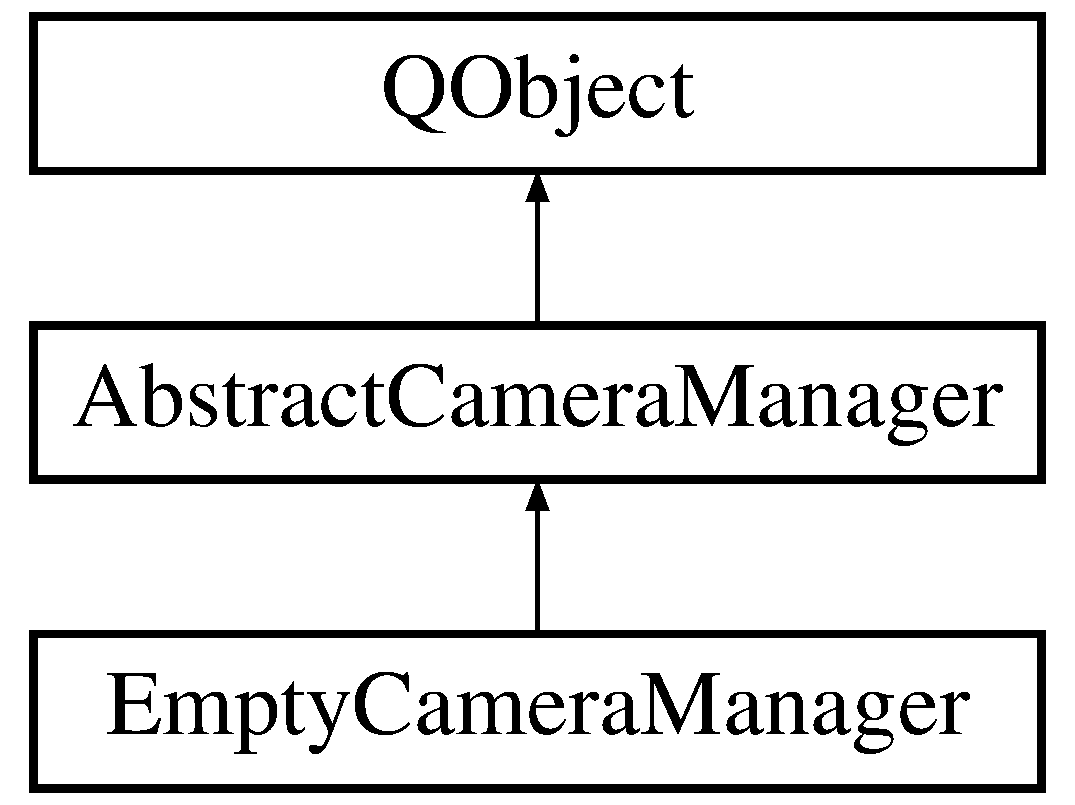
\includegraphics[height=3.000000cm]{class_empty_camera_manager}
\end{center}
\end{figure}
\subsection*{Public Member Functions}
\begin{DoxyCompactItemize}
\item 
virtual void \hyperlink{class_empty_camera_manager_ae32a44d1576763cf49d46dba3aef0007}{detect\-New\-Cameras} (std\-::vector$<$ \hyperlink{class_abstract_camera}{Abstract\-Camera} $\ast$ $>$ $\ast$)
\begin{DoxyCompactList}\small\item\em detect\-New\-Cameras (Pure virtual) detect new cameras \end{DoxyCompactList}\item 
\hypertarget{class_empty_camera_manager_a321c93993d5bdd065f9ea875ee7b7961}{virtual void {\bfseries get\-Cameras\-Properties\-List} () const }\label{class_empty_camera_manager_a321c93993d5bdd065f9ea875ee7b7961}

\item 
virtual std\-::string \hyperlink{class_empty_camera_manager_acd29e9bb06b9839e5c94b6ffe5ee86a9}{get\-Name} () const 
\begin{DoxyCompactList}\small\item\em get\-Name (Pure virtual) get the name of the Manager \end{DoxyCompactList}\end{DoxyCompactItemize}
\subsection*{Additional Inherited Members}


\subsection{Member Function Documentation}
\hypertarget{class_empty_camera_manager_ae32a44d1576763cf49d46dba3aef0007}{\index{Empty\-Camera\-Manager@{Empty\-Camera\-Manager}!detect\-New\-Cameras@{detect\-New\-Cameras}}
\index{detect\-New\-Cameras@{detect\-New\-Cameras}!EmptyCameraManager@{Empty\-Camera\-Manager}}
\subsubsection[{detect\-New\-Cameras}]{\setlength{\rightskip}{0pt plus 5cm}void Empty\-Camera\-Manager\-::detect\-New\-Cameras (
\begin{DoxyParamCaption}
\item[{std\-::vector$<$ {\bf Abstract\-Camera} $\ast$ $>$ $\ast$}]{new\-Cameras}
\end{DoxyParamCaption}
)\hspace{0.3cm}{\ttfamily [virtual]}}}\label{class_empty_camera_manager_ae32a44d1576763cf49d46dba3aef0007}


detect\-New\-Cameras (Pure virtual) detect new cameras 


\begin{DoxyParams}{Parameters}
{\em new\-Cameras} & wich will need to be filled with all the camera connected to the computer \\
\hline
\end{DoxyParams}


Implements \hyperlink{class_abstract_camera_manager_a8e215b2531fd8c18551382dc8f571817}{Abstract\-Camera\-Manager}.

\hypertarget{class_empty_camera_manager_acd29e9bb06b9839e5c94b6ffe5ee86a9}{\index{Empty\-Camera\-Manager@{Empty\-Camera\-Manager}!get\-Name@{get\-Name}}
\index{get\-Name@{get\-Name}!EmptyCameraManager@{Empty\-Camera\-Manager}}
\subsubsection[{get\-Name}]{\setlength{\rightskip}{0pt plus 5cm}std\-::string Empty\-Camera\-Manager\-::get\-Name (
\begin{DoxyParamCaption}
{}
\end{DoxyParamCaption}
) const\hspace{0.3cm}{\ttfamily [virtual]}}}\label{class_empty_camera_manager_acd29e9bb06b9839e5c94b6ffe5ee86a9}


get\-Name (Pure virtual) get the name of the Manager 

\begin{DoxyReturn}{Returns}
String containing the name manager 
\end{DoxyReturn}


Implements \hyperlink{class_abstract_camera_manager_a6e4b041842471b9ed42ddd5c9ab260d1}{Abstract\-Camera\-Manager}.



The documentation for this class was generated from the following files\-:\begin{DoxyCompactItemize}
\item 
C\-:/\-Users/\-V1rgul/\-Git\-Hub/\-Project-\/\-Norway/\-Projet\-Norvege/emptycameramanager.\-h\item 
C\-:/\-Users/\-V1rgul/\-Git\-Hub/\-Project-\/\-Norway/\-Projet\-Norvege/emptycameramanager.\-cpp\end{DoxyCompactItemize}

\hypertarget{class_fly_camera}{\section{Fly\-Camera Class Reference}
\label{class_fly_camera}\index{Fly\-Camera@{Fly\-Camera}}
}


The \hyperlink{class_fly_camera}{Fly\-Camera} class, represent a Fly\-Capture Camera with all its settings.  




{\ttfamily \#include $<$flycamera.\-h$>$}

Inheritance diagram for Fly\-Camera\-:\begin{figure}[H]
\begin{center}
\leavevmode
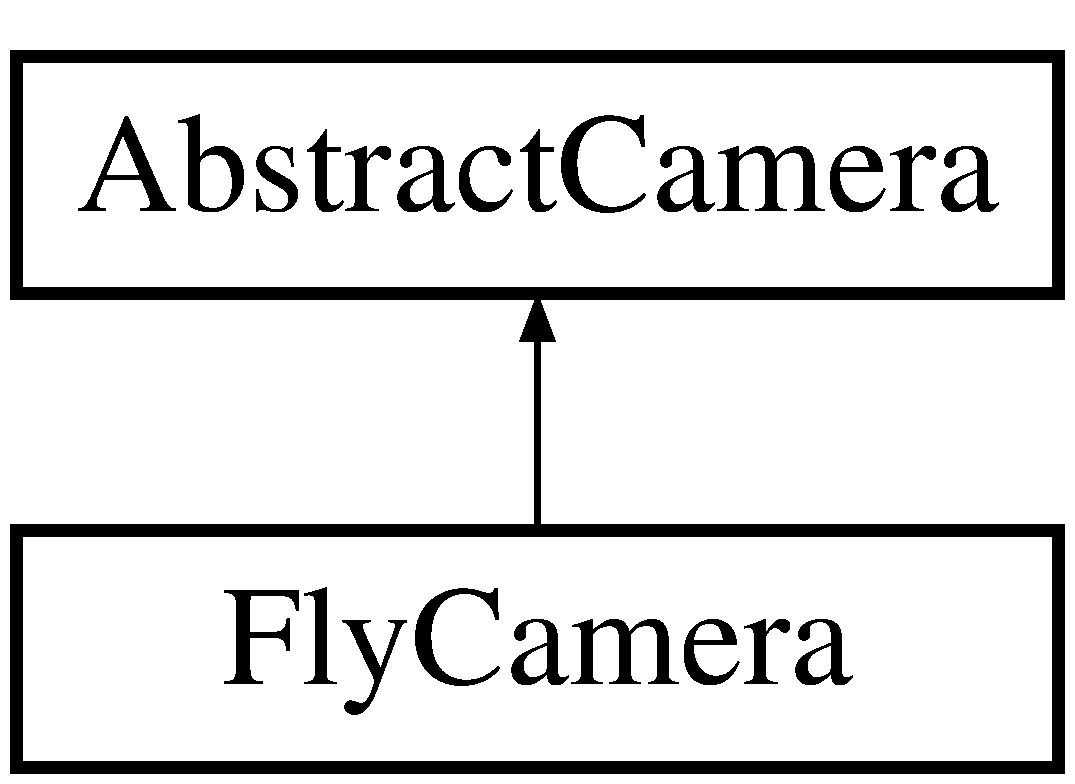
\includegraphics[height=2.000000cm]{class_fly_camera}
\end{center}
\end{figure}
\subsection*{Public Member Functions}
\begin{DoxyCompactItemize}
\item 
\hypertarget{class_fly_camera_a3176768aac0905151237c2e9633c8c47}{Camera $\ast$ {\bfseries get\-Camera} ()}\label{class_fly_camera_a3176768aac0905151237c2e9633c8c47}

\item 
\hypertarget{class_fly_camera_ae5b32f2f930f8903fde35a5aeeb059b6}{P\-G\-R\-Guid $\ast$ {\bfseries get\-Guid} ()}\label{class_fly_camera_ae5b32f2f930f8903fde35a5aeeb059b6}

\item 
\hypertarget{class_fly_camera_abfba126bfff4fee7042710451b198286}{Camera\-Info $\ast$ {\bfseries get\-Camera\-Info} ()}\label{class_fly_camera_abfba126bfff4fee7042710451b198286}

\item 
void \hyperlink{class_fly_camera_ad9d4102cab167f0d5739b2af808c43ee}{set\-Property} (\hyperlink{class_camera_manager_1_1_camera_property}{Camera\-Manager\-::\-Camera\-Property} $\ast$p)
\begin{DoxyCompactList}\small\item\em (Pure virtual) set the camera according to that property \end{DoxyCompactList}\item 
void \hyperlink{class_fly_camera_a8f87a0d8ccbee558e629189e2c8ab271}{update\-Property} (\hyperlink{class_camera_manager_1_1_camera_property}{Camera\-Manager\-::\-Camera\-Property} $\ast$p)
\begin{DoxyCompactList}\small\item\em (Pure virtual) get the value of that property for that camera \end{DoxyCompactList}\item 
\hypertarget{class_fly_camera_aa91c2cd580029a1fb242e2d8dace33b7}{void \hyperlink{class_fly_camera_aa91c2cd580029a1fb242e2d8dace33b7}{start\-Auto\-Capture} ()}\label{class_fly_camera_aa91c2cd580029a1fb242e2d8dace33b7}

\begin{DoxyCompactList}\small\item\em (Pure virtual) start callback based Liveview \end{DoxyCompactList}\item 
\hypertarget{class_fly_camera_a7d637bd9237fae3ee3cd55b044ec80f1}{void \hyperlink{class_fly_camera_a7d637bd9237fae3ee3cd55b044ec80f1}{stop\-Auto\-Capture} ()}\label{class_fly_camera_a7d637bd9237fae3ee3cd55b044ec80f1}

\begin{DoxyCompactList}\small\item\em (Pure virtual) stop\-Auto\-Capture stop callback based Liveview \end{DoxyCompactList}\item 
Q\-Image \hyperlink{class_fly_camera_a0e935d2f7d21e31e470670ff5b6740e1}{retrieve\-Image} ()
\begin{DoxyCompactList}\small\item\em (Pure virtual) get one image from camera \end{DoxyCompactList}\item 
bool \hyperlink{class_fly_camera_a8121735229105485f73289a36bd41042}{equals\-To} (\hyperlink{class_abstract_camera}{Abstract\-Camera} $\ast$c)
\begin{DoxyCompactList}\small\item\em compare 2 cameras \end{DoxyCompactList}\item 
std\-::string \hyperlink{class_fly_camera_a97938fec7396d02574383f7db50d9e58}{get\-String} ()
\begin{DoxyCompactList}\small\item\em (Pure virtual) get the name corresponding to the camera model and id \end{DoxyCompactList}\end{DoxyCompactItemize}
\subsection*{Additional Inherited Members}


\subsection{Detailed Description}
The \hyperlink{class_fly_camera}{Fly\-Camera} class, represent a Fly\-Capture Camera with all its settings. 

\subsection{Member Function Documentation}
\hypertarget{class_fly_camera_a8121735229105485f73289a36bd41042}{\index{Fly\-Camera@{Fly\-Camera}!equals\-To@{equals\-To}}
\index{equals\-To@{equals\-To}!FlyCamera@{Fly\-Camera}}
\subsubsection[{equals\-To}]{\setlength{\rightskip}{0pt plus 5cm}bool Fly\-Camera\-::equals\-To (
\begin{DoxyParamCaption}
\item[{{\bf Abstract\-Camera} $\ast$}]{c}
\end{DoxyParamCaption}
)\hspace{0.3cm}{\ttfamily [virtual]}}}\label{class_fly_camera_a8121735229105485f73289a36bd41042}


compare 2 cameras 


\begin{DoxyParams}{Parameters}
{\em c} & camera to compare \\
\hline
\end{DoxyParams}
\begin{DoxyReturn}{Returns}
true if the cameras are physically the same 
\end{DoxyReturn}


Reimplemented from \hyperlink{class_abstract_camera_a244917ab081c18caf389473847871dd6}{Abstract\-Camera}.

\hypertarget{class_fly_camera_a97938fec7396d02574383f7db50d9e58}{\index{Fly\-Camera@{Fly\-Camera}!get\-String@{get\-String}}
\index{get\-String@{get\-String}!FlyCamera@{Fly\-Camera}}
\subsubsection[{get\-String}]{\setlength{\rightskip}{0pt plus 5cm}std\-::string Fly\-Camera\-::get\-String (
\begin{DoxyParamCaption}
{}
\end{DoxyParamCaption}
)\hspace{0.3cm}{\ttfamily [virtual]}}}\label{class_fly_camera_a97938fec7396d02574383f7db50d9e58}


(Pure virtual) get the name corresponding to the camera model and id 

\begin{DoxyReturn}{Returns}
String containing these informations 
\end{DoxyReturn}


Implements \hyperlink{class_abstract_camera_a75dc6b53d5a8717944d5e8ded9609611}{Abstract\-Camera}.

\hypertarget{class_fly_camera_a0e935d2f7d21e31e470670ff5b6740e1}{\index{Fly\-Camera@{Fly\-Camera}!retrieve\-Image@{retrieve\-Image}}
\index{retrieve\-Image@{retrieve\-Image}!FlyCamera@{Fly\-Camera}}
\subsubsection[{retrieve\-Image}]{\setlength{\rightskip}{0pt plus 5cm}Q\-Image Fly\-Camera\-::retrieve\-Image (
\begin{DoxyParamCaption}
{}
\end{DoxyParamCaption}
)\hspace{0.3cm}{\ttfamily [virtual]}}}\label{class_fly_camera_a0e935d2f7d21e31e470670ff5b6740e1}


(Pure virtual) get one image from camera 

\begin{DoxyReturn}{Returns}
Q\-Image image 
\end{DoxyReturn}


Implements \hyperlink{class_abstract_camera_aec58ab298b618632fd422cadd11bae17}{Abstract\-Camera}.

\hypertarget{class_fly_camera_ad9d4102cab167f0d5739b2af808c43ee}{\index{Fly\-Camera@{Fly\-Camera}!set\-Property@{set\-Property}}
\index{set\-Property@{set\-Property}!FlyCamera@{Fly\-Camera}}
\subsubsection[{set\-Property}]{\setlength{\rightskip}{0pt plus 5cm}void Fly\-Camera\-::set\-Property (
\begin{DoxyParamCaption}
\item[{{\bf Camera\-Manager\-::\-Camera\-Property} $\ast$}]{p}
\end{DoxyParamCaption}
)\hspace{0.3cm}{\ttfamily [virtual]}}}\label{class_fly_camera_ad9d4102cab167f0d5739b2af808c43ee}


(Pure virtual) set the camera according to that property 


\begin{DoxyParams}{Parameters}
{\em p} & property to set \\
\hline
\end{DoxyParams}


Implements \hyperlink{class_abstract_camera_a8b50d3e4925cfe74ed383376ba02bb5e}{Abstract\-Camera}.

\hypertarget{class_fly_camera_a8f87a0d8ccbee558e629189e2c8ab271}{\index{Fly\-Camera@{Fly\-Camera}!update\-Property@{update\-Property}}
\index{update\-Property@{update\-Property}!FlyCamera@{Fly\-Camera}}
\subsubsection[{update\-Property}]{\setlength{\rightskip}{0pt plus 5cm}void Fly\-Camera\-::update\-Property (
\begin{DoxyParamCaption}
\item[{{\bf Camera\-Manager\-::\-Camera\-Property} $\ast$}]{p}
\end{DoxyParamCaption}
)\hspace{0.3cm}{\ttfamily [virtual]}}}\label{class_fly_camera_a8f87a0d8ccbee558e629189e2c8ab271}


(Pure virtual) get the value of that property for that camera 


\begin{DoxyParams}{Parameters}
{\em p} & property to update \\
\hline
\end{DoxyParams}


Implements \hyperlink{class_abstract_camera_acb48ab701cd02e78604a3ca1c695b1cf}{Abstract\-Camera}.



The documentation for this class was generated from the following files\-:\begin{DoxyCompactItemize}
\item 
C\-:/\-Users/\-V1rgul/\-Git\-Hub/\-Project-\/\-Norway/\-Projet\-Norvege/flycamera.\-h\item 
C\-:/\-Users/\-V1rgul/\-Git\-Hub/\-Project-\/\-Norway/\-Projet\-Norvege/flycamera.\-cpp\end{DoxyCompactItemize}

\hypertarget{class_fly_camera_manager}{\section{Fly\-Camera\-Manager Class Reference}
\label{class_fly_camera_manager}\index{Fly\-Camera\-Manager@{Fly\-Camera\-Manager}}
}


The \hyperlink{class_fly_camera_manager}{Fly\-Camera\-Manager} class deals with all the Fly Capture Cameras.  




{\ttfamily \#include $<$flycameramanager.\-h$>$}

Inheritance diagram for Fly\-Camera\-Manager\-:\begin{figure}[H]
\begin{center}
\leavevmode
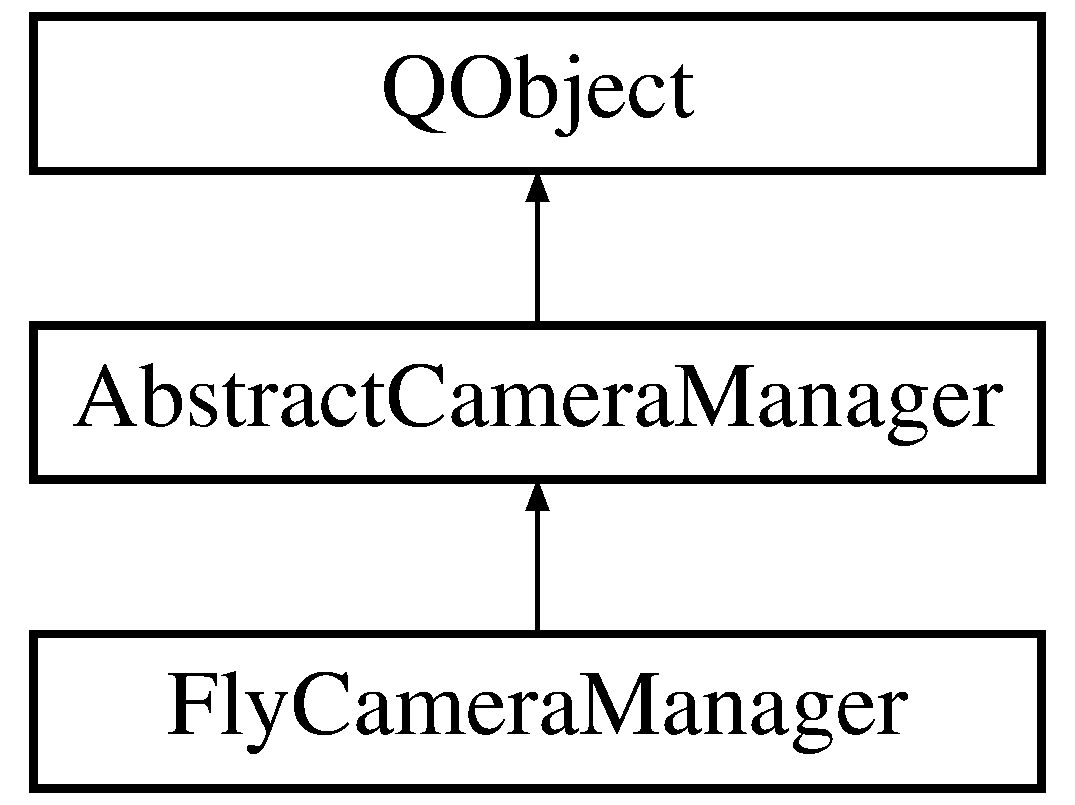
\includegraphics[height=3.000000cm]{class_fly_camera_manager}
\end{center}
\end{figure}
\subsection*{Public Member Functions}
\begin{DoxyCompactItemize}
\item 
virtual void \hyperlink{class_fly_camera_manager_aab72966a50baaf966817c7f1265341a8}{detect\-New\-Cameras} (std\-::vector$<$ \hyperlink{class_abstract_camera}{Abstract\-Camera} $\ast$ $>$ $\ast$new\-Cameras)
\begin{DoxyCompactList}\small\item\em (Pure virtual) detect new cameras \end{DoxyCompactList}\item 
std\-::string \hyperlink{class_fly_camera_manager_a1c865e44bde9cc91829c3e875081396d}{get\-Name} () const 
\begin{DoxyCompactList}\small\item\em (Pure virtual) get the name of the Manager \end{DoxyCompactList}\end{DoxyCompactItemize}
\subsection*{Additional Inherited Members}


\subsection{Detailed Description}
The \hyperlink{class_fly_camera_manager}{Fly\-Camera\-Manager} class deals with all the Fly Capture Cameras. 

\subsection{Member Function Documentation}
\hypertarget{class_fly_camera_manager_aab72966a50baaf966817c7f1265341a8}{\index{Fly\-Camera\-Manager@{Fly\-Camera\-Manager}!detect\-New\-Cameras@{detect\-New\-Cameras}}
\index{detect\-New\-Cameras@{detect\-New\-Cameras}!FlyCameraManager@{Fly\-Camera\-Manager}}
\subsubsection[{detect\-New\-Cameras}]{\setlength{\rightskip}{0pt plus 5cm}void Fly\-Camera\-Manager\-::detect\-New\-Cameras (
\begin{DoxyParamCaption}
\item[{std\-::vector$<$ {\bf Abstract\-Camera} $\ast$ $>$ $\ast$}]{new\-Cameras}
\end{DoxyParamCaption}
)\hspace{0.3cm}{\ttfamily [virtual]}}}\label{class_fly_camera_manager_aab72966a50baaf966817c7f1265341a8}


(Pure virtual) detect new cameras 


\begin{DoxyParams}{Parameters}
{\em new\-Cameras} & (modified by the function) will be filled with all the camera connected to the computer, even ones already connected \\
\hline
\end{DoxyParams}


Implements \hyperlink{class_abstract_camera_manager_a8e215b2531fd8c18551382dc8f571817}{Abstract\-Camera\-Manager}.

\hypertarget{class_fly_camera_manager_a1c865e44bde9cc91829c3e875081396d}{\index{Fly\-Camera\-Manager@{Fly\-Camera\-Manager}!get\-Name@{get\-Name}}
\index{get\-Name@{get\-Name}!FlyCameraManager@{Fly\-Camera\-Manager}}
\subsubsection[{get\-Name}]{\setlength{\rightskip}{0pt plus 5cm}string Fly\-Camera\-Manager\-::get\-Name (
\begin{DoxyParamCaption}
{}
\end{DoxyParamCaption}
) const\hspace{0.3cm}{\ttfamily [virtual]}}}\label{class_fly_camera_manager_a1c865e44bde9cc91829c3e875081396d}


(Pure virtual) get the name of the Manager 

\begin{DoxyReturn}{Returns}
String containing the name manager 
\end{DoxyReturn}


Implements \hyperlink{class_abstract_camera_manager_a6e4b041842471b9ed42ddd5c9ab260d1}{Abstract\-Camera\-Manager}.



The documentation for this class was generated from the following files\-:\begin{DoxyCompactItemize}
\item 
C\-:/\-Users/\-V1rgul/\-Git\-Hub/\-Project-\/\-Norway/\-Projet\-Norvege/flycameramanager.\-h\item 
C\-:/\-Users/\-V1rgul/\-Git\-Hub/\-Project-\/\-Norway/\-Projet\-Norvege/flycameramanager.\-cpp\end{DoxyCompactItemize}

\hypertarget{class_is_camera}{\section{Is\-Camera Class Reference}
\label{class_is_camera}\index{Is\-Camera@{Is\-Camera}}
}


The \hyperlink{class_is_camera}{Is\-Camera} class, represent a Image Source Camera with all its settings.  




{\ttfamily \#include $<$iscamera.\-h$>$}

Inheritance diagram for Is\-Camera\-:\begin{figure}[H]
\begin{center}
\leavevmode
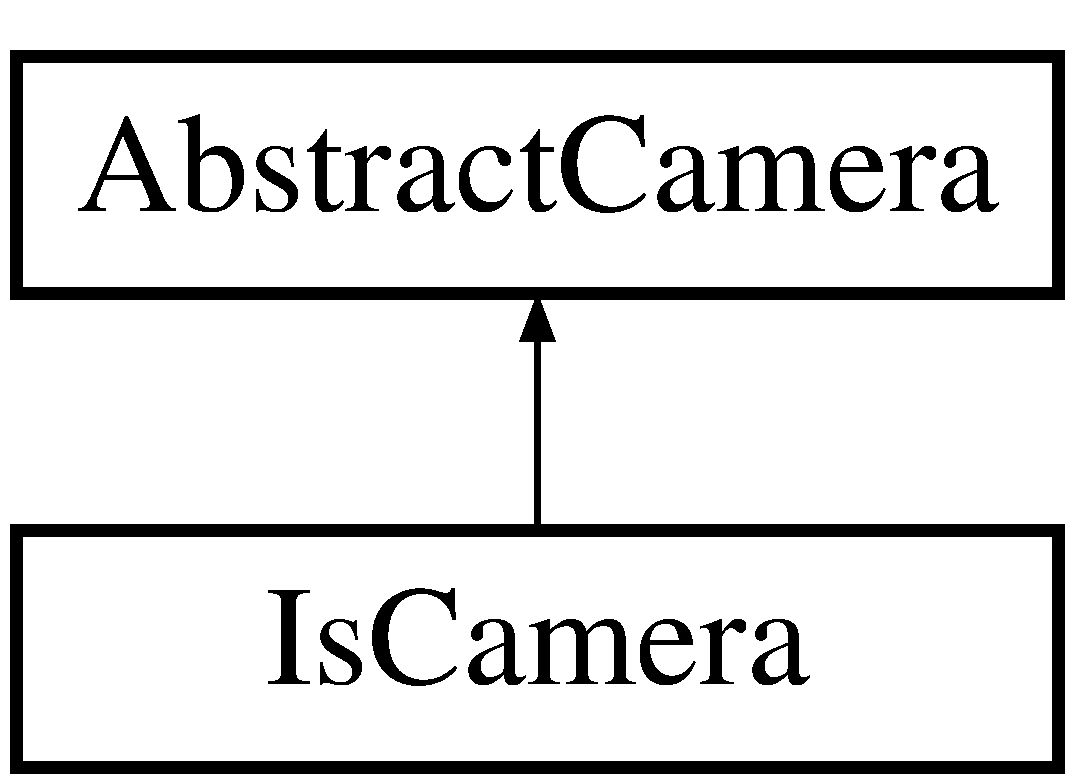
\includegraphics[height=2.000000cm]{class_is_camera}
\end{center}
\end{figure}
\subsection*{Public Member Functions}
\begin{DoxyCompactItemize}
\item 
\hypertarget{class_is_camera_ab1f39bed7530f03cf07c3ae6c53d045e}{Camera $\ast$ {\bfseries get\-Camera} ()}\label{class_is_camera_ab1f39bed7530f03cf07c3ae6c53d045e}

\item 
\hypertarget{class_is_camera_a08a1845f52db3f52fae52aa2ce63783b}{P\-G\-R\-Guid $\ast$ {\bfseries get\-Guid} ()}\label{class_is_camera_a08a1845f52db3f52fae52aa2ce63783b}

\item 
\hypertarget{class_is_camera_acfd929b7612162a9897f0be21b2bea4f}{Camera\-Info $\ast$ {\bfseries get\-Camera\-Info} ()}\label{class_is_camera_acfd929b7612162a9897f0be21b2bea4f}

\item 
void \hyperlink{class_is_camera_a70c90a32bde9fcc3c594a526c7cba33c}{set\-Property} (\hyperlink{class_camera_manager_1_1_camera_property}{Camera\-Manager\-::\-Camera\-Property} $\ast$p)
\begin{DoxyCompactList}\small\item\em set\-Property set the camera according to that property \end{DoxyCompactList}\item 
void \hyperlink{class_is_camera_a5e2c484168c627eb79d61658e880300d}{update\-Property} (\hyperlink{class_camera_manager_1_1_camera_property}{Camera\-Manager\-::\-Camera\-Property} $\ast$p)
\begin{DoxyCompactList}\small\item\em update\-Property get the value of that property for that camera \end{DoxyCompactList}\item 
\hypertarget{class_is_camera_ad272b7a566ab9d226c96b331a0e8b5ab}{void \hyperlink{class_is_camera_ad272b7a566ab9d226c96b331a0e8b5ab}{start\-Auto\-Capture} ()}\label{class_is_camera_ad272b7a566ab9d226c96b331a0e8b5ab}

\begin{DoxyCompactList}\small\item\em start\-Auto\-Capture start callback based Liveview \end{DoxyCompactList}\item 
\hypertarget{class_is_camera_a71a1959c599bb6f296dc59965a41b8c7}{void \hyperlink{class_is_camera_a71a1959c599bb6f296dc59965a41b8c7}{stop\-Auto\-Capture} ()}\label{class_is_camera_a71a1959c599bb6f296dc59965a41b8c7}

\begin{DoxyCompactList}\small\item\em stop\-Auto\-Capture stop callback based Liveview \end{DoxyCompactList}\item 
\hypertarget{class_is_camera_acc1229819c8d296c6f25cb358f6e1650}{void {\bfseries send\-Frame} (Q\-Image img)}\label{class_is_camera_acc1229819c8d296c6f25cb358f6e1650}

\item 
Q\-Image \hyperlink{class_is_camera_abd737cee4788d70a4614d8ea6ea883d2}{retrieve\-Image} ()
\begin{DoxyCompactList}\small\item\em retrieve\-Image get one image from camera \end{DoxyCompactList}\item 
bool \hyperlink{class_is_camera_acb734c645fa0c5e4ffc64001b87daa0d}{equals\-To} (\hyperlink{class_abstract_camera}{Abstract\-Camera} $\ast$c)
\begin{DoxyCompactList}\small\item\em equals\-To compare 2 cameras \end{DoxyCompactList}\item 
std\-::string \hyperlink{class_is_camera_af0791bc3cdb5d552fb6f73285b467408}{get\-String} ()
\begin{DoxyCompactList}\small\item\em get\-String get the name corresponding to the camera model and id \end{DoxyCompactList}\end{DoxyCompactItemize}
\subsection*{Additional Inherited Members}


\subsection{Detailed Description}
The \hyperlink{class_is_camera}{Is\-Camera} class, represent a Image Source Camera with all its settings. 

\subsection{Member Function Documentation}
\hypertarget{class_is_camera_acb734c645fa0c5e4ffc64001b87daa0d}{\index{Is\-Camera@{Is\-Camera}!equals\-To@{equals\-To}}
\index{equals\-To@{equals\-To}!IsCamera@{Is\-Camera}}
\subsubsection[{equals\-To}]{\setlength{\rightskip}{0pt plus 5cm}bool Is\-Camera\-::equals\-To (
\begin{DoxyParamCaption}
\item[{{\bf Abstract\-Camera} $\ast$}]{c}
\end{DoxyParamCaption}
)\hspace{0.3cm}{\ttfamily [virtual]}}}\label{class_is_camera_acb734c645fa0c5e4ffc64001b87daa0d}


equals\-To compare 2 cameras 


\begin{DoxyParams}{Parameters}
{\em c} & camera to compare \\
\hline
\end{DoxyParams}
\begin{DoxyReturn}{Returns}
true if the cameras are physically the same 
\end{DoxyReturn}


Reimplemented from \hyperlink{class_abstract_camera_a244917ab081c18caf389473847871dd6}{Abstract\-Camera}.

\hypertarget{class_is_camera_af0791bc3cdb5d552fb6f73285b467408}{\index{Is\-Camera@{Is\-Camera}!get\-String@{get\-String}}
\index{get\-String@{get\-String}!IsCamera@{Is\-Camera}}
\subsubsection[{get\-String}]{\setlength{\rightskip}{0pt plus 5cm}std\-::string Is\-Camera\-::get\-String (
\begin{DoxyParamCaption}
{}
\end{DoxyParamCaption}
)\hspace{0.3cm}{\ttfamily [virtual]}}}\label{class_is_camera_af0791bc3cdb5d552fb6f73285b467408}


get\-String get the name corresponding to the camera model and id 

\begin{DoxyReturn}{Returns}
String containing these informations 
\end{DoxyReturn}


Implements \hyperlink{class_abstract_camera_a75dc6b53d5a8717944d5e8ded9609611}{Abstract\-Camera}.

\hypertarget{class_is_camera_abd737cee4788d70a4614d8ea6ea883d2}{\index{Is\-Camera@{Is\-Camera}!retrieve\-Image@{retrieve\-Image}}
\index{retrieve\-Image@{retrieve\-Image}!IsCamera@{Is\-Camera}}
\subsubsection[{retrieve\-Image}]{\setlength{\rightskip}{0pt plus 5cm}Q\-Image Is\-Camera\-::retrieve\-Image (
\begin{DoxyParamCaption}
{}
\end{DoxyParamCaption}
)\hspace{0.3cm}{\ttfamily [virtual]}}}\label{class_is_camera_abd737cee4788d70a4614d8ea6ea883d2}


retrieve\-Image get one image from camera 

\begin{DoxyReturn}{Returns}
Q\-Image image 
\end{DoxyReturn}


Implements \hyperlink{class_abstract_camera_aec58ab298b618632fd422cadd11bae17}{Abstract\-Camera}.

\hypertarget{class_is_camera_a70c90a32bde9fcc3c594a526c7cba33c}{\index{Is\-Camera@{Is\-Camera}!set\-Property@{set\-Property}}
\index{set\-Property@{set\-Property}!IsCamera@{Is\-Camera}}
\subsubsection[{set\-Property}]{\setlength{\rightskip}{0pt plus 5cm}void Is\-Camera\-::set\-Property (
\begin{DoxyParamCaption}
\item[{{\bf Camera\-Manager\-::\-Camera\-Property} $\ast$}]{p}
\end{DoxyParamCaption}
)\hspace{0.3cm}{\ttfamily [virtual]}}}\label{class_is_camera_a70c90a32bde9fcc3c594a526c7cba33c}


set\-Property set the camera according to that property 


\begin{DoxyParams}{Parameters}
{\em p} & property to set \\
\hline
\end{DoxyParams}


Implements \hyperlink{class_abstract_camera_a8b50d3e4925cfe74ed383376ba02bb5e}{Abstract\-Camera}.

\hypertarget{class_is_camera_a5e2c484168c627eb79d61658e880300d}{\index{Is\-Camera@{Is\-Camera}!update\-Property@{update\-Property}}
\index{update\-Property@{update\-Property}!IsCamera@{Is\-Camera}}
\subsubsection[{update\-Property}]{\setlength{\rightskip}{0pt plus 5cm}void Is\-Camera\-::update\-Property (
\begin{DoxyParamCaption}
\item[{{\bf Camera\-Manager\-::\-Camera\-Property} $\ast$}]{p}
\end{DoxyParamCaption}
)\hspace{0.3cm}{\ttfamily [virtual]}}}\label{class_is_camera_a5e2c484168c627eb79d61658e880300d}


update\-Property get the value of that property for that camera 


\begin{DoxyParams}{Parameters}
{\em p} & property to update \\
\hline
\end{DoxyParams}


Implements \hyperlink{class_abstract_camera_acb48ab701cd02e78604a3ca1c695b1cf}{Abstract\-Camera}.



The documentation for this class was generated from the following files\-:\begin{DoxyCompactItemize}
\item 
C\-:/\-Users/\-V1rgul/\-Git\-Hub/\-Project-\/\-Norway/\-Projet\-Norvege/iscamera.\-h\item 
C\-:/\-Users/\-V1rgul/\-Git\-Hub/\-Project-\/\-Norway/\-Projet\-Norvege/iscamera.\-cpp\end{DoxyCompactItemize}

\hypertarget{class_is_camera_manager}{\section{Is\-Camera\-Manager Class Reference}
\label{class_is_camera_manager}\index{Is\-Camera\-Manager@{Is\-Camera\-Manager}}
}


The \hyperlink{class_fly_camera_manager}{Fly\-Camera\-Manager} class deals with all the Fly Capture Cameras.  




{\ttfamily \#include $<$iscameramanager.\-h$>$}

Inheritance diagram for Is\-Camera\-Manager\-:\begin{figure}[H]
\begin{center}
\leavevmode
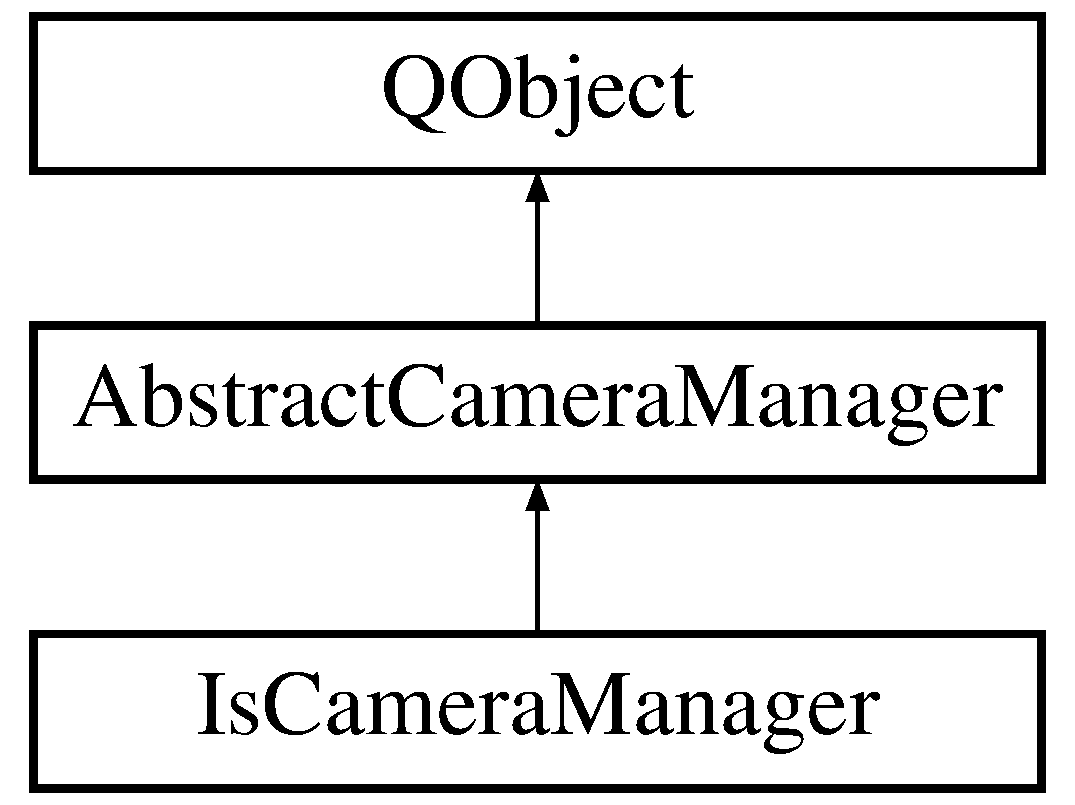
\includegraphics[height=3.000000cm]{class_is_camera_manager}
\end{center}
\end{figure}
\subsection*{Public Member Functions}
\begin{DoxyCompactItemize}
\item 
virtual void \hyperlink{class_is_camera_manager_a4b65e770537668dffca47cbf6af34dfb}{detect\-New\-Cameras} (std\-::vector$<$ \hyperlink{class_abstract_camera}{Abstract\-Camera} $\ast$ $>$ $\ast$new\-Cameras)
\begin{DoxyCompactList}\small\item\em detect\-New\-Cameras (Pure virtual) detect new cameras \end{DoxyCompactList}\item 
std\-::string \hyperlink{class_is_camera_manager_a86228372c8903914acc3764e9358163b}{get\-Name} () const 
\begin{DoxyCompactList}\small\item\em get\-Name (Pure virtual) get the name of the Manager \end{DoxyCompactList}\item 
\hypertarget{class_is_camera_manager_a505c0eef8802a84ecc777112d4fcdc32}{void {\bfseries get\-Cameras\-Properties\-List} () const }\label{class_is_camera_manager_a505c0eef8802a84ecc777112d4fcdc32}

\end{DoxyCompactItemize}
\subsection*{Public Attributes}
\begin{DoxyCompactItemize}
\item 
\hypertarget{class_is_camera_manager_a526b595eafb56059b9f8a5fc5d2d5d89}{unsigned int {\bfseries num\-Cameras}}\label{class_is_camera_manager_a526b595eafb56059b9f8a5fc5d2d5d89}

\end{DoxyCompactItemize}
\subsection*{Additional Inherited Members}


\subsection{Detailed Description}
The \hyperlink{class_fly_camera_manager}{Fly\-Camera\-Manager} class deals with all the Fly Capture Cameras. 

\subsection{Member Function Documentation}
\hypertarget{class_is_camera_manager_a4b65e770537668dffca47cbf6af34dfb}{\index{Is\-Camera\-Manager@{Is\-Camera\-Manager}!detect\-New\-Cameras@{detect\-New\-Cameras}}
\index{detect\-New\-Cameras@{detect\-New\-Cameras}!IsCameraManager@{Is\-Camera\-Manager}}
\subsubsection[{detect\-New\-Cameras}]{\setlength{\rightskip}{0pt plus 5cm}void Is\-Camera\-Manager\-::detect\-New\-Cameras (
\begin{DoxyParamCaption}
\item[{std\-::vector$<$ {\bf Abstract\-Camera} $\ast$ $>$ $\ast$}]{new\-Cameras}
\end{DoxyParamCaption}
)\hspace{0.3cm}{\ttfamily [virtual]}}}\label{class_is_camera_manager_a4b65e770537668dffca47cbf6af34dfb}


detect\-New\-Cameras (Pure virtual) detect new cameras 


\begin{DoxyParams}{Parameters}
{\em new\-Cameras} & wich will need to be filled with all the camera connected to the computer \\
\hline
\end{DoxyParams}


Implements \hyperlink{class_abstract_camera_manager_a8e215b2531fd8c18551382dc8f571817}{Abstract\-Camera\-Manager}.

\hypertarget{class_is_camera_manager_a86228372c8903914acc3764e9358163b}{\index{Is\-Camera\-Manager@{Is\-Camera\-Manager}!get\-Name@{get\-Name}}
\index{get\-Name@{get\-Name}!IsCameraManager@{Is\-Camera\-Manager}}
\subsubsection[{get\-Name}]{\setlength{\rightskip}{0pt plus 5cm}string Is\-Camera\-Manager\-::get\-Name (
\begin{DoxyParamCaption}
{}
\end{DoxyParamCaption}
) const\hspace{0.3cm}{\ttfamily [virtual]}}}\label{class_is_camera_manager_a86228372c8903914acc3764e9358163b}


get\-Name (Pure virtual) get the name of the Manager 

\begin{DoxyReturn}{Returns}
String containing the name manager 
\end{DoxyReturn}


Implements \hyperlink{class_abstract_camera_manager_a6e4b041842471b9ed42ddd5c9ab260d1}{Abstract\-Camera\-Manager}.



The documentation for this class was generated from the following files\-:\begin{DoxyCompactItemize}
\item 
C\-:/\-Users/\-V1rgul/\-Git\-Hub/\-Project-\/\-Norway/\-Projet\-Norvege/iscameramanager.\-h\item 
C\-:/\-Users/\-V1rgul/\-Git\-Hub/\-Project-\/\-Norway/\-Projet\-Norvege/iscameramanager.\-cpp\end{DoxyCompactItemize}

\hypertarget{class_main_window}{\section{Main\-Window Class Reference}
\label{class_main_window}\index{Main\-Window@{Main\-Window}}
}
Inheritance diagram for Main\-Window\-:\begin{figure}[H]
\begin{center}
\leavevmode
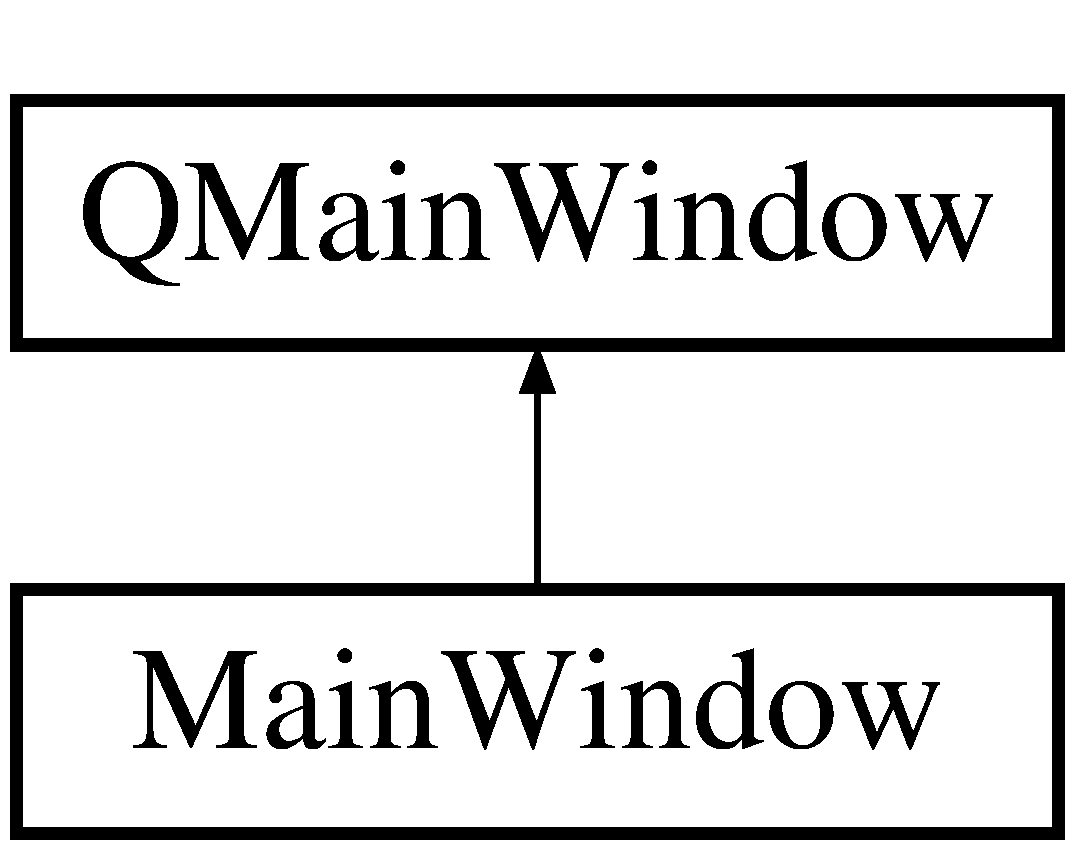
\includegraphics[height=2.000000cm]{class_main_window}
\end{center}
\end{figure}
\subsection*{Signals}
\begin{DoxyCompactItemize}
\item 
\hypertarget{class_main_window_a8aca5460ce992afb3fcba398cc387466}{void {\bfseries activate\-Crosshair} (bool)}\label{class_main_window_a8aca5460ce992afb3fcba398cc387466}

\end{DoxyCompactItemize}
\subsection*{Public Member Functions}
\begin{DoxyCompactItemize}
\item 
\hypertarget{class_main_window_a8b244be8b7b7db1b08de2a2acb9409db}{{\bfseries Main\-Window} (Q\-Widget $\ast$parent=0)}\label{class_main_window_a8b244be8b7b7db1b08de2a2acb9409db}

\item 
\hypertarget{class_main_window_aa1aedeaf20f2f0b571a7bd655e3e819e}{void {\bfseries modify\-Sub\-Window} (Q\-Mdi\-Sub\-Window $\ast$in, bool add)}\label{class_main_window_aa1aedeaf20f2f0b571a7bd655e3e819e}

\end{DoxyCompactItemize}


The documentation for this class was generated from the following files\-:\begin{DoxyCompactItemize}
\item 
C\-:/\-Users/\-V1rgul/\-Git\-Hub/\-Project-\/\-Norway/\-Projet\-Norvege/mainwindow.\-h\item 
C\-:/\-Users/\-V1rgul/\-Git\-Hub/\-Project-\/\-Norway/\-Projet\-Norvege/mainwindow.\-cpp\end{DoxyCompactItemize}

\hypertarget{class_q_video_widget}{\section{Q\-Video\-Widget Class Reference}
\label{class_q_video_widget}\index{Q\-Video\-Widget@{Q\-Video\-Widget}}
}
Inheritance diagram for Q\-Video\-Widget\-:\begin{figure}[H]
\begin{center}
\leavevmode
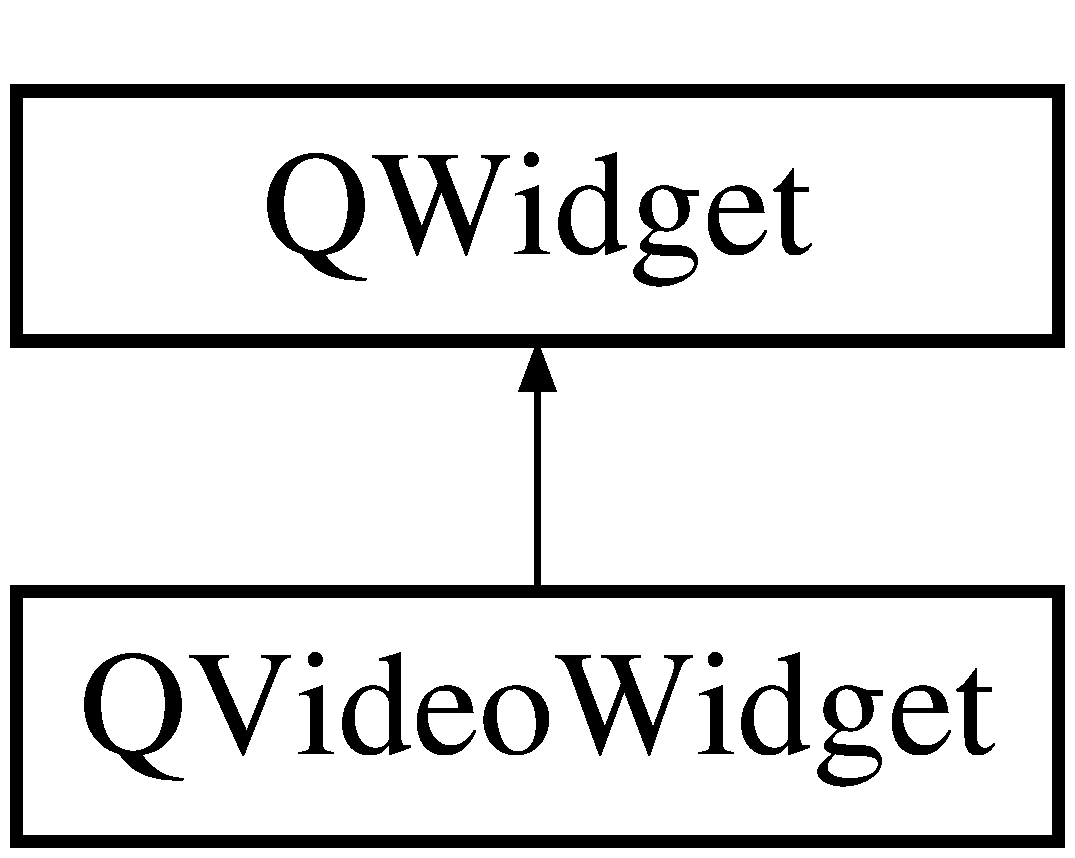
\includegraphics[height=2.000000cm]{class_q_video_widget}
\end{center}
\end{figure}
\subsection*{Public Slots}
\begin{DoxyCompactItemize}
\item 
\hypertarget{class_q_video_widget_aa3be10b5a18667fe60b6da0deba33e2b}{void {\bfseries changed\-State} (Qt\-::\-Window\-States old\-State, Qt\-::\-Window\-States new\-State)}\label{class_q_video_widget_aa3be10b5a18667fe60b6da0deba33e2b}

\item 
\hypertarget{class_q_video_widget_a35f34cdbb0f92307698c02b2dc99c4bd}{void {\bfseries activate\-Crosshair} (bool state)}\label{class_q_video_widget_a35f34cdbb0f92307698c02b2dc99c4bd}

\item 
\hypertarget{class_q_video_widget_a12b2bc7e23dd56adff244520acf4d16c}{void {\bfseries receive\-Update} ()}\label{class_q_video_widget_a12b2bc7e23dd56adff244520acf4d16c}

\end{DoxyCompactItemize}
\subsection*{Signals}
\begin{DoxyCompactItemize}
\item 
\hypertarget{class_q_video_widget_a7669505f07e3d66ea9a0c1553c096ea2}{void {\bfseries force\-Update} ()}\label{class_q_video_widget_a7669505f07e3d66ea9a0c1553c096ea2}

\end{DoxyCompactItemize}
\subsection*{Public Member Functions}
\begin{DoxyCompactItemize}
\item 
\hypertarget{class_q_video_widget_a9556e8daac0717d705ac8c2fd7e4e2a2}{{\bfseries Q\-Video\-Widget} (Q\-Widget $\ast$parent=0)}\label{class_q_video_widget_a9556e8daac0717d705ac8c2fd7e4e2a2}

\item 
\hypertarget{class_q_video_widget_a331955ccf1e82259702db3fc15983eff}{void {\bfseries set\-Image} (Q\-Image image)}\label{class_q_video_widget_a331955ccf1e82259702db3fc15983eff}

\end{DoxyCompactItemize}
\subsection*{Protected Member Functions}
\begin{DoxyCompactItemize}
\item 
\hypertarget{class_q_video_widget_afa241c4f57f7198f4625b9ac42fbaa79}{void {\bfseries paint\-Event} (Q\-Paint\-Event $\ast$event)}\label{class_q_video_widget_afa241c4f57f7198f4625b9ac42fbaa79}

\item 
\hypertarget{class_q_video_widget_a935858a83ef55740c9424870dc652962}{void {\bfseries resize\-Event} (Q\-Resize\-Event $\ast$event=N\-U\-L\-L)}\label{class_q_video_widget_a935858a83ef55740c9424870dc652962}

\item 
\hypertarget{class_q_video_widget_ab04e47a7d99ee39b6d459bfc94c0b0b0}{void {\bfseries mouse\-Move\-Event} (Q\-Mouse\-Event $\ast$event)}\label{class_q_video_widget_ab04e47a7d99ee39b6d459bfc94c0b0b0}

\item 
\hypertarget{class_q_video_widget_a4c1e806be89ef42a8e5a7771115b886f}{void {\bfseries leave\-Event} (Q\-Event $\ast$)}\label{class_q_video_widget_a4c1e806be89ef42a8e5a7771115b886f}

\end{DoxyCompactItemize}


The documentation for this class was generated from the following files\-:\begin{DoxyCompactItemize}
\item 
C\-:/\-Users/\-V1rgul/\-Git\-Hub/\-Project-\/\-Norway/\-Projet\-Norvege/qvideowidget.\-h\item 
C\-:/\-Users/\-V1rgul/\-Git\-Hub/\-Project-\/\-Norway/\-Projet\-Norvege/qvideowidget.\-cpp\end{DoxyCompactItemize}

\hypertarget{class_test_camera}{\section{Test\-Camera Class Reference}
\label{class_test_camera}\index{Test\-Camera@{Test\-Camera}}
}


to test ui without real cameras.  




{\ttfamily \#include $<$testcamera.\-h$>$}

Inheritance diagram for Test\-Camera\-:\begin{figure}[H]
\begin{center}
\leavevmode
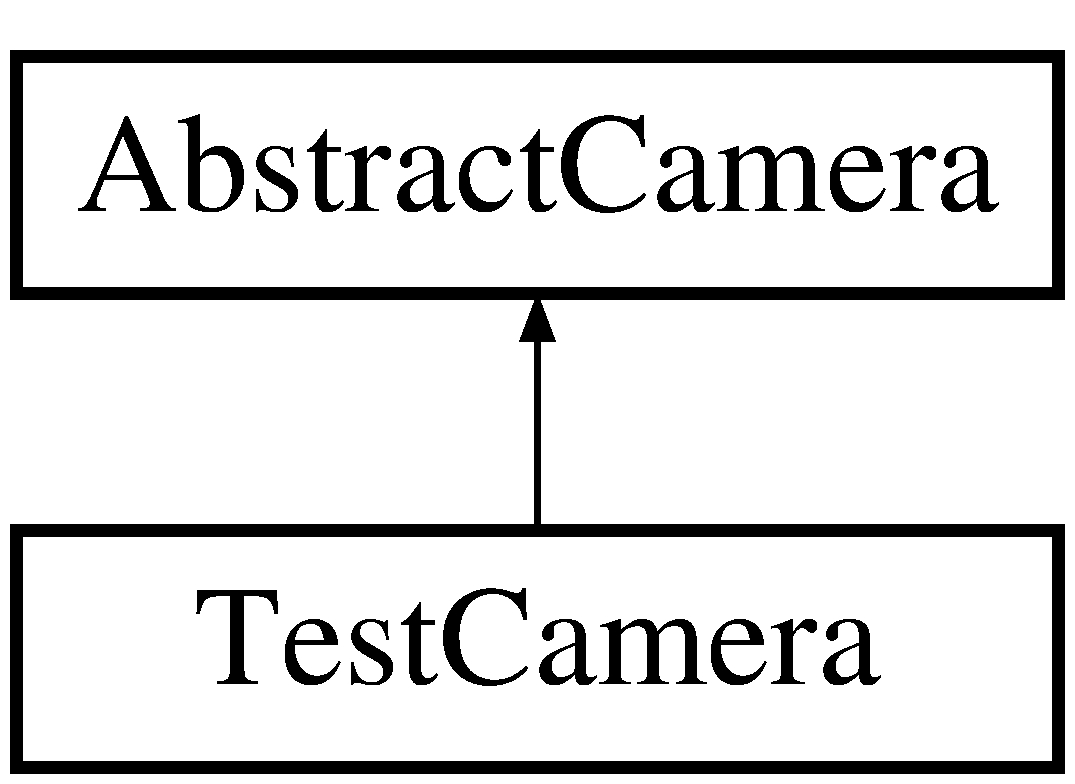
\includegraphics[height=2.000000cm]{class_test_camera}
\end{center}
\end{figure}
\subsection*{Public Member Functions}
\begin{DoxyCompactItemize}
\item 
\hypertarget{class_test_camera_a46fb8a67d24675886760e6fc0058edb3}{{\bfseries Test\-Camera} (std\-::string n)}\label{class_test_camera_a46fb8a67d24675886760e6fc0058edb3}

\item 
void \hyperlink{class_test_camera_a92507f0e4601f93912b06297e4b59d99}{set\-Property} (\hyperlink{class_camera_manager_1_1_camera_property}{Camera\-Property} $\ast$p)
\begin{DoxyCompactList}\small\item\em (Pure virtual) set the camera according to that property \end{DoxyCompactList}\item 
void \hyperlink{class_test_camera_a6b0c9e25baafe0a8d211b32851cb67b3}{update\-Property} (\hyperlink{class_camera_manager_1_1_camera_property}{Camera\-Property} $\ast$p)
\begin{DoxyCompactList}\small\item\em (Pure virtual) get the value of that property for that camera \end{DoxyCompactList}\item 
std\-::string \hyperlink{class_test_camera_a5ddb007a4c0c44e06b24787298f1c97c}{get\-String} ()
\begin{DoxyCompactList}\small\item\em (Pure virtual) get the name corresponding to the camera model and id \end{DoxyCompactList}\item 
Q\-Image \hyperlink{class_test_camera_a283bd75f1b9500e35ba7aa252c2df14e}{retrieve\-Image} ()
\begin{DoxyCompactList}\small\item\em (Pure virtual) get one image from camera \end{DoxyCompactList}\item 
\hypertarget{class_test_camera_a095498b65800c150009292e73f765621}{void \hyperlink{class_test_camera_a095498b65800c150009292e73f765621}{start\-Auto\-Capture} ()}\label{class_test_camera_a095498b65800c150009292e73f765621}

\begin{DoxyCompactList}\small\item\em (Pure virtual) start callback based Liveview \end{DoxyCompactList}\item 
\hypertarget{class_test_camera_a52f8f0ee49d83d927878cc2dd64a0af1}{void \hyperlink{class_test_camera_a52f8f0ee49d83d927878cc2dd64a0af1}{stop\-Auto\-Capture} ()}\label{class_test_camera_a52f8f0ee49d83d927878cc2dd64a0af1}

\begin{DoxyCompactList}\small\item\em (Pure virtual) stop\-Auto\-Capture stop callback based Liveview \end{DoxyCompactList}\end{DoxyCompactItemize}
\subsection*{Additional Inherited Members}


\subsection{Detailed Description}
to test ui without real cameras. 

\hyperlink{class_test_camera}{Test\-Camera} 

\subsection{Member Function Documentation}
\hypertarget{class_test_camera_a5ddb007a4c0c44e06b24787298f1c97c}{\index{Test\-Camera@{Test\-Camera}!get\-String@{get\-String}}
\index{get\-String@{get\-String}!TestCamera@{Test\-Camera}}
\subsubsection[{get\-String}]{\setlength{\rightskip}{0pt plus 5cm}std\-::string Test\-Camera\-::get\-String (
\begin{DoxyParamCaption}
{}
\end{DoxyParamCaption}
)\hspace{0.3cm}{\ttfamily [inline]}, {\ttfamily [virtual]}}}\label{class_test_camera_a5ddb007a4c0c44e06b24787298f1c97c}


(Pure virtual) get the name corresponding to the camera model and id 

\begin{DoxyReturn}{Returns}
String containing these informations 
\end{DoxyReturn}


Implements \hyperlink{class_abstract_camera_a75dc6b53d5a8717944d5e8ded9609611}{Abstract\-Camera}.

\hypertarget{class_test_camera_a283bd75f1b9500e35ba7aa252c2df14e}{\index{Test\-Camera@{Test\-Camera}!retrieve\-Image@{retrieve\-Image}}
\index{retrieve\-Image@{retrieve\-Image}!TestCamera@{Test\-Camera}}
\subsubsection[{retrieve\-Image}]{\setlength{\rightskip}{0pt plus 5cm}Q\-Image Test\-Camera\-::retrieve\-Image (
\begin{DoxyParamCaption}
{}
\end{DoxyParamCaption}
)\hspace{0.3cm}{\ttfamily [virtual]}}}\label{class_test_camera_a283bd75f1b9500e35ba7aa252c2df14e}


(Pure virtual) get one image from camera 

\begin{DoxyReturn}{Returns}
Q\-Image image 
\end{DoxyReturn}


Implements \hyperlink{class_abstract_camera_aec58ab298b618632fd422cadd11bae17}{Abstract\-Camera}.

\hypertarget{class_test_camera_a92507f0e4601f93912b06297e4b59d99}{\index{Test\-Camera@{Test\-Camera}!set\-Property@{set\-Property}}
\index{set\-Property@{set\-Property}!TestCamera@{Test\-Camera}}
\subsubsection[{set\-Property}]{\setlength{\rightskip}{0pt plus 5cm}void Test\-Camera\-::set\-Property (
\begin{DoxyParamCaption}
\item[{{\bf Camera\-Property} $\ast$}]{p}
\end{DoxyParamCaption}
)\hspace{0.3cm}{\ttfamily [virtual]}}}\label{class_test_camera_a92507f0e4601f93912b06297e4b59d99}


(Pure virtual) set the camera according to that property 


\begin{DoxyParams}{Parameters}
{\em p} & property to set \\
\hline
\end{DoxyParams}


Implements \hyperlink{class_abstract_camera_a8b50d3e4925cfe74ed383376ba02bb5e}{Abstract\-Camera}.

\hypertarget{class_test_camera_a6b0c9e25baafe0a8d211b32851cb67b3}{\index{Test\-Camera@{Test\-Camera}!update\-Property@{update\-Property}}
\index{update\-Property@{update\-Property}!TestCamera@{Test\-Camera}}
\subsubsection[{update\-Property}]{\setlength{\rightskip}{0pt plus 5cm}void Test\-Camera\-::update\-Property (
\begin{DoxyParamCaption}
\item[{{\bf Camera\-Property} $\ast$}]{p}
\end{DoxyParamCaption}
)\hspace{0.3cm}{\ttfamily [virtual]}}}\label{class_test_camera_a6b0c9e25baafe0a8d211b32851cb67b3}


(Pure virtual) get the value of that property for that camera 


\begin{DoxyParams}{Parameters}
{\em p} & property to update \\
\hline
\end{DoxyParams}


Implements \hyperlink{class_abstract_camera_acb48ab701cd02e78604a3ca1c695b1cf}{Abstract\-Camera}.



The documentation for this class was generated from the following files\-:\begin{DoxyCompactItemize}
\item 
C\-:/\-Users/\-V1rgul/\-Git\-Hub/\-Project-\/\-Norway/\-Projet\-Norvege/\hyperlink{testcamera_8h}{testcamera.\-h}\item 
C\-:/\-Users/\-V1rgul/\-Git\-Hub/\-Project-\/\-Norway/\-Projet\-Norvege/testcamera.\-cpp\end{DoxyCompactItemize}

\hypertarget{class_test_camera_manager}{\section{Test\-Camera\-Manager Class Reference}
\label{class_test_camera_manager}\index{Test\-Camera\-Manager@{Test\-Camera\-Manager}}
}
Inheritance diagram for Test\-Camera\-Manager\-:\begin{figure}[H]
\begin{center}
\leavevmode
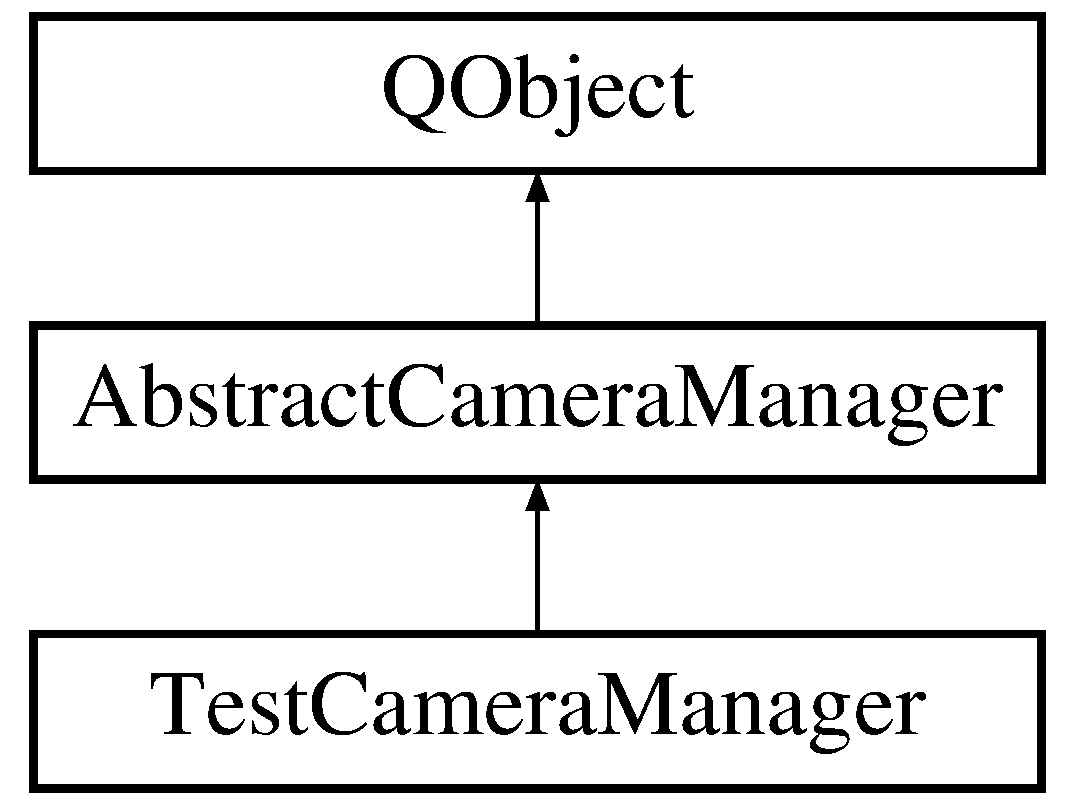
\includegraphics[height=3.000000cm]{class_test_camera_manager}
\end{center}
\end{figure}
\subsection*{Public Member Functions}
\begin{DoxyCompactItemize}
\item 
virtual void \hyperlink{class_test_camera_manager_a06c6f51030a289253f2ea214d1475c26}{detect\-New\-Cameras} (std\-::vector$<$ \hyperlink{class_abstract_camera}{Abstract\-Camera} $\ast$ $>$ $\ast$new\-Cameras)
\begin{DoxyCompactList}\small\item\em (Pure virtual) detect new cameras \end{DoxyCompactList}\item 
virtual std\-::string \hyperlink{class_test_camera_manager_adb2da700417695044c0bf1ba2ab21cf3}{get\-Name} () const 
\begin{DoxyCompactList}\small\item\em (Pure virtual) get the name of the Manager \end{DoxyCompactList}\end{DoxyCompactItemize}
\subsection*{Additional Inherited Members}


\subsection{Member Function Documentation}
\hypertarget{class_test_camera_manager_a06c6f51030a289253f2ea214d1475c26}{\index{Test\-Camera\-Manager@{Test\-Camera\-Manager}!detect\-New\-Cameras@{detect\-New\-Cameras}}
\index{detect\-New\-Cameras@{detect\-New\-Cameras}!TestCameraManager@{Test\-Camera\-Manager}}
\subsubsection[{detect\-New\-Cameras}]{\setlength{\rightskip}{0pt plus 5cm}void Test\-Camera\-Manager\-::detect\-New\-Cameras (
\begin{DoxyParamCaption}
\item[{std\-::vector$<$ {\bf Abstract\-Camera} $\ast$ $>$ $\ast$}]{new\-Cameras}
\end{DoxyParamCaption}
)\hspace{0.3cm}{\ttfamily [virtual]}}}\label{class_test_camera_manager_a06c6f51030a289253f2ea214d1475c26}


(Pure virtual) detect new cameras 


\begin{DoxyParams}{Parameters}
{\em new\-Cameras} & (modified by the function) will be filled with all the camera connected to the computer, even ones already connected \\
\hline
\end{DoxyParams}


Implements \hyperlink{class_abstract_camera_manager_a8e215b2531fd8c18551382dc8f571817}{Abstract\-Camera\-Manager}.

\hypertarget{class_test_camera_manager_adb2da700417695044c0bf1ba2ab21cf3}{\index{Test\-Camera\-Manager@{Test\-Camera\-Manager}!get\-Name@{get\-Name}}
\index{get\-Name@{get\-Name}!TestCameraManager@{Test\-Camera\-Manager}}
\subsubsection[{get\-Name}]{\setlength{\rightskip}{0pt plus 5cm}std\-::string Test\-Camera\-Manager\-::get\-Name (
\begin{DoxyParamCaption}
{}
\end{DoxyParamCaption}
) const\hspace{0.3cm}{\ttfamily [virtual]}}}\label{class_test_camera_manager_adb2da700417695044c0bf1ba2ab21cf3}


(Pure virtual) get the name of the Manager 

\begin{DoxyReturn}{Returns}
String containing the name manager 
\end{DoxyReturn}


Implements \hyperlink{class_abstract_camera_manager_a6e4b041842471b9ed42ddd5c9ab260d1}{Abstract\-Camera\-Manager}.



The documentation for this class was generated from the following files\-:\begin{DoxyCompactItemize}
\item 
C\-:/\-Users/\-V1rgul/\-Git\-Hub/\-Project-\/\-Norway/\-Projet\-Norvege/testcameramanager.\-h\item 
C\-:/\-Users/\-V1rgul/\-Git\-Hub/\-Project-\/\-Norway/\-Projet\-Norvege/testcameramanager.\-cpp\end{DoxyCompactItemize}

%--- End generated contents ---

% Index
\newpage
\phantomsection
\addcontentsline{toc}{part}{Index}
\printindex

\end{document}
